\chapter{CPU、存储器、芯片引脚与完整计算机}

\begin{keyidea}
CPU 不是“什么都能做的黑盒”，ROM 也不是“放代码的神秘区域”。处理器通过
引脚和平台互连发出地址、方向与数据事务，地址译码选择 RAM、非易失存储或
设备；取指、译码、执行和提交只是这些部件按时序合作的结果。
\end{keyidea}

\section{芯片封装、引脚、ISA 与 CPU 结构}

\term{die}{裸片}是在晶圆上制造并切割出的半导体区域；它包含晶体管、互连和
片上存储。\term{package}{封装}保护裸片并把微小焊盘转换成可装配的外部焊盘
或引脚。\term{chip}{芯片}在日常语境中常指已经封装的器件。\term{module}
{模块}可以把处理器、内存、Flash 和电源管理等多个器件装在一块小板上；
\term{carrier board}{载板}再提供连接器、供电和外围接口。

\begin{pdfdiagram}
  \node[os hardware] (die) {硅裸片 die\\晶体管与片上互连};
  \node[os hardware,right=of die] (package) {封装 package\\焊球/引脚};
  \node[os hardware,right=of package] (module) {计算模块\\芯片与无源元件};
  \node[os hardware,right=of module] (board) {载板/主板\\接口与电源};
  \draw[os arrow] (die) -- node[above]{键合/倒装} (package);
  \draw[os arrow] (package) -- node[above]{焊接} (module);
  \draw[os arrow] (module) -- node[above]{板间连接} (board);
\end{pdfdiagram}

“CPU 有多少个引脚”不是只数地址线。现代封装中大量焊球用于多个电源域和地，
其余还承担内存通道、PCIe、显示、时钟、复位、调试、配置和保留功能。

\topic{芯片引脚的六类职责}
\begin{osgridlongtable}{L{0.16\linewidth}L{0.32\linewidth}L{0.42\linewidth}}
类别 & 例子 & 为什么需要 \\ \hline
\endfirsthead
类别 & 例子 & 为什么需要 \\ \hline
\endhead
电源与地 & VCC、VDD、VSS、GND & 输送能量、建立参考和低阻回流 \\ \hline
时钟与复位 & CLK、RESET\_N、PWRGOOD & 规定时序并建立已知初态 \\ \hline
数据 & DQ、TX/RX、MOSI/MISO & 传送有效载荷 \\ \hline
地址与选择 & A[\,]、CS\_N、BA[\,] & 选择芯片、存储体或位置 \\ \hline
控制与状态 & RD\_N、WR\_N、READY、IRQ & 描述方向、完成、错误和事件 \\ \hline
配置与测试 & strap、JTAG、保留脚 & 选择启动配置、制造测试与调试 \\ \hline
\end{osgridlongtable}

\begin{center}
\begin{tikzpicture}[font=\scriptsize\sffamily]
  \draw[rounded corners=3pt,draw=BookBlue,fill=BookCodeBg]
    (-3.2,-2.3) rectangle (3.2,2.3);
  \node[font=\bfseries] at (0,0) {概念 CPU/SoC 封装顶视};
  \foreach \x/\name in {-2.4/VDD,-1.2/GND,0/VDD,1.2/GND,2.4/VDD}
    \node[os pin] at (\x,2.65) {\name};
  \foreach \x/\name in {-2.4/CLK,-1.2/RESET\_N,0/PWRGOOD,1.2/JTAG,2.4/GND}
    \node[os pin] at (\x,-2.65) {\name};
  \foreach \y/\name in {1.65/A0,0.9/A1,0.15/CS\_N,-0.6/RD\_N,-1.35/WR\_N}
    \node[os pin] at (-3.65,\y) {\name};
  \foreach \y/\name in {1.65/D0,0.9/D1,0.15/D2,-0.6/D3,-1.35/IRQ}
    \node[os pin] at (3.65,\y) {\name};
  \draw[fill=BookAmber] (-2.85,1.85) circle (0.11);
  \node[BookMuted] at (-2.1,1.85) {pin 1 标记};
\end{tikzpicture}
\end{center}
\diagramnote{这是一张教学引脚图，不对应具体处理器。真实 BGA 常有数百至上千
焊球，必须使用厂商 pin list、封装图和电源设计指南，不能照此图接线。}

\topic{CPU 的承诺分为架构与微架构}
\term{指令集架构}{instruction set architecture, ISA}规定软件可见寄存器、
指令编码、地址计算、异常与特权等契约。\term{微架构}{microarchitecture}
规定某颗 CPU 内部怎样用流水线、执行单元、缓存和预测器实现这些契约。

两个处理器可以都执行 x86-64 程序，却具有不同缓存大小、流水线深度和执行
吞吐。操作系统可以利用 CPUID 等架构接口发现部分能力，但不应依赖未承诺的
内部节点。

\begin{osgridlongtable}{L{0.20\linewidth}L{0.33\linewidth}L{0.37\linewidth}}
层次 & 对软件承诺 & 例子 \\ \hline
\endfirsthead
层次 & 对软件承诺 & 例子 \\ \hline
\endhead
ISA & 必须长期兼容的软件可见行为 & RAX、RIP、ADD、MOV、页表、异常向量 \\ \hline
微架构 & 在 ISA 允许范围内选择实现 & 乱序窗口、执行端口、缓存替换、分支预测 \\ \hline
平台 & CPU 外围地址与设备组织 & ROM 映射、RAM 窗口、UART/ATA/PIC \\ \hline
电路板 & 真实供电、封装和连线 & 电源轨、晶振、Flash、PCB 差分对 \\ \hline
\end{osgridlongtable}

\topic{一颗教学 CPU 至少需要哪些部分}
\begin{pdfdiagram}[node distance=8mm and 8mm]
  \node[BookMuted,font=\bfseries] (control-label) {控制链};
  \node[os state,right=of control-label,minimum width=24mm] (pc)
    {程序计数器\\给出取指地址};
  \node[os hardware,right=of pc,minimum width=24mm] (imem)
    {指令接口\\返回机器码};
  \node[os block,right=of imem,minimum width=24mm] (decode)
    {译码与控制\\形成控制信号};
  \draw[os bus] (pc) -- node[above]{地址} (imem);
  \draw[os bus] (imem) -- node[above]{指令字节} (decode);

  \node[BookMuted,font=\bfseries,below=13mm of control-label] (data-label)
    {数据链};
  \node[os state,right=of data-label,minimum width=24mm] (regs)
    {寄存器文件\\读出操作数};
  \node[os block,right=of regs,minimum width=24mm] (alu)
    {ALU\\计算值或地址};
  \node[os hardware,right=of alu,minimum width=24mm] (dmem)
    {数据接口\\访问 RAM/设备};
  \draw[os bus] (regs) -- node[above]{操作数} (alu);
  \draw[os bus] (alu) -- node[above]{值/地址} (dmem);

  \draw[os arrow,dashed] (decode.south) --
    node[right]{选择、使能、读写} (dmem.north);
  \draw[os arrow,dashed] (decode.south west) --
    node[left]{ALU 操作} (alu.north);
\end{pdfdiagram}
\diagramnote{上泳道决定“做什么”，下泳道搬运并变换“对什么做”。写回寄存器、
更新标志和选择下一条 PC 都发生在本次指令提交处；为避免交叉线，提交反馈在下一幅
逐周期数据通路图中展开。}

真实现代 CPU 会把取指、译码、重命名、调度、执行和退休重叠，还会把复杂
x86 指令转换成内部微操作。但从 ISA 观察，处理器仍要产生与顺序规则一致的
架构结果或精确异常。

\topic{取指、译码、执行、访存和提交}
教学上可把一条指令分成五个逻辑阶段：

\begin{enumerate}[leftmargin=2.2em]
  \item \textbf{取指：}用 RIP/PC 给出的地址请求机器码字节；
  \item \textbf{译码：}识别操作码、寄存器、立即数、长度和权限要求；
  \item \textbf{执行：}由 ALU 或其他单元计算结果或有效地址；
  \item \textbf{访存：}若需要，对缓存、RAM 或设备发起事务；
  \item \textbf{提交：}更新软件可见寄存器、标志和下一指令地址，或提交异常。
\end{enumerate}

\begin{workedexample}
假设一台简化 CPU 执行“把寄存器 \(R_1\) 与 \(R_2\) 相加写入 \(R_3\)”：

\[
R_1=7,\qquad R_2=5.
\]

译码器选择两个读端口和 ALU 的 ADD 功能；ALU 形成 \(12\)；时钟边沿允许
寄存器 \(R_3\leftarrow12\)；PC 增加指令长度。若位宽为 4 bit，结果仍是
\(1100_2\)；若计算 \(15+3=18\)，4-bit 结果只保存 \(0010_2\)，并产生
进位条件。CPU 执行的是固定宽度状态转换，不是无限精度数学。
\end{workedexample}

\section{指令周期、数据通路与流水线}

\term{冯·诺依曼式}{von Neumann}组织让指令和数据共享一个可寻址存储体系；
\term{Harvard 式}{Harvard}组织为指令和数据提供分离存储或接口。现代 CPU
常表现为混合结构：软件看到统一虚拟地址空间，内部却有分离的 L1 指令缓存和
数据缓存，更下层再汇合。

\begin{osgridlongtable}{L{0.19\linewidth}L{0.31\linewidth}L{0.40\linewidth}}
组织 & 优势 & 代价与现实变体 \\ \hline
\endfirsthead
组织 & 优势 & 代价与现实变体 \\ \hline
\endhead
统一存储 & 指令和数据可共享容量，程序易装载修改 & 取指与数据访问争用同一通路 \\ \hline
分离存储 & 可同时取指和访数据，权限/宽度可不同 & 两边容量固定，交换内容需要额外机制 \\ \hline
现代混合 & ISA 统一、近端缓存分离、下层汇合 & 必须维护指令/数据缓存与修改代码的一致性 \\ \hline
\end{osgridlongtable}

“程序也是 byte”表示指令可以存储和搬运，不表示 CPU 会把任意数据自动执行。
取指必须来自当前控制流选择的地址，并通过执行权限、模式和译码规则。

\topic{把 CPU 打开：数据通路与控制通路分别做什么}
\term{数据通路}{datapath}搬运并变换值，包括寄存器文件、ALU、多路选择器和
总线；\term{控制通路}{control path}根据指令、状态和条件产生选择、读写、
使能与下一状态。

\begin{center}
\begin{tikzpicture}[font=\footnotesize\sffamily,>=Latex]
  \node[os state,minimum width=23mm] (pc) at (0,4.6) {PC/RIP\\取指地址};
  \node[os hardware,minimum width=25mm] (memory) at (3.5,4.6)
    {指令存储接口\\返回机器码};
  \node[os state,minimum width=23mm] (ir) at (7.0,4.6)
    {指令寄存器 IR\\当前编码};
  \node[os block,minimum width=27mm] (decode) at (10.5,4.6)
    {译码/控制器\\产生控制信号};

  \node[os state,minimum width=28mm] (regs) at (0.5,1.5)
    {寄存器文件\\两个读口、一个写口};
  \node[os block,minimum width=28mm] (operands) at (4.0,1.5)
    {操作数选择\\MUX A / MUX B};
  \node[os block,minimum width=27mm] (alu) at (7.4,1.5)
    {ALU\\算术/地址/逻辑};
  \node[os state,minimum width=25mm] (result) at (10.5,1.5)
    {结果与标志};

  \draw[os bus] (pc) -- (memory);
  \draw[os bus] (memory) -- (ir);
  \draw[os bus] (ir) -- (decode);
  \draw[os bus] ([yshift=2mm]regs.east) -- ([yshift=2mm]operands.west);
  \draw[os bus] ([yshift=-2mm]regs.east) -- ([yshift=-2mm]operands.west);
  \draw[os bus] (operands) -- (alu);
  \draw[os bus] (alu) -- (result);

  \draw[os arrow,BookTeal] (decode.south) --
    node[right]{提交使能} (result.north);
  \draw[os arrow,BookTeal] ([xshift=-4mm]decode.south) -- ++(0,-0.55) -|
    node[pos=0.30,above]{选择与运算控制} (operands.north);

  \draw[os bus] (result.south) -- ++(0,-1.0) -|
    node[pos=0.45,below]{写回} (regs.south);
  \draw[os arrow] (result.east) -- ++(0.65,0) |- ++(0,4.2) -|
    node[pos=0.45,above]{顺序、分支或异常决定下一 RIP} (pc.north);
\end{tikzpicture}
\end{center}
\diagramnote{蓝色双线表示多 bit 数据，绿色细线表示控制选择。这是一张教学
数据通路；真实 x86 核心还包含乱序执行、预测、缓存等结构，几何位置也不同。}

\topic{寄存器文件为什么常有多个端口}
一条二操作数算术指令通常要同时读取两个源，再写一个目标。寄存器文件可提供
两个组合读端口和一个时钟写端口。地址译码选择寄存器，读多路选择器返回内容，
写使能只在提交时更新目标。

\begin{center}
\begin{tikzpicture}[font=\footnotesize\sffamily,>=Latex]
  \draw[rounded corners=3pt,draw=BookBlue,fill=BookCodeBg]
    (3,0) rectangle (8,4.8);
  \node[font=\bfseries] at (5.5,4.3) {寄存器文件};
  \foreach \y/\name in {3.4/R0,2.7/R1,2.0/R2,1.3/\(\cdots\),0.6/R15}
    \node[draw=BookRule,fill=white,minimum width=18mm,minimum height=5mm]
      at (5.5,\y) {\name};
  \node[os state] (ra) at (0,3.6) {read addr A};
  \node[os state] (rb) at (0,2.4) {read addr B};
  \node[os state] (wa) at (0,1.2) {write addr};
  \node[os state] (wd) at (5.5,-1.0) {write data + enable};
  \node[os state] (qa) at (11,3.3) {read data A};
  \node[os state] (qb) at (11,1.6) {read data B};
  \draw[os arrow] (ra) -- (3,3.6);
  \draw[os arrow] (rb) -- (3,2.4);
  \draw[os arrow] (wa) -- (3,1.2);
  \draw[os bus] (wd) -- (5.5,0);
  \draw[os bus] (8,3.3) -- (qa);
  \draw[os bus] (8,1.6) -- (qb);
\end{tikzpicture}
\end{center}

\topic{机器指令包含“做什么”和“对谁做”}
机器指令编码通常要表达部分或全部字段：

\begin{itemize}[leftmargin=2.2em]
  \item opcode：ADD、LOAD、JUMP 等操作；
  \item 源/目标寄存器编号；
  \item 立即数或位移；
  \item 寻址方式、操作数宽度和条件；
  \item 某些 ISA 中的权限或扩展前缀。
\end{itemize}

为建立直觉，定义一套\textbf{纯教学、不是 x86} 的 16-bit 定长指令。所有
指令都占 2 byte，最高 4 bit 是 opcode，其余字段随指令种类解释：

\begin{center}
\begin{tikzpicture}[font=\footnotesize\sffamily]
  \foreach \x/\w/\colorname/\title/\bits in {
    0/3.2/BookBlue/opcode/\(15..12\),
    3.2/3.2/BookTeal/字段 A/\(11..8\),
    6.4/6.4/BookAmber/字段 B/\(7..0\)} {
    \fill[\colorname!18] (\x,0) rectangle ++(\w,1.15);
    \draw[\colorname,thick] (\x,0) rectangle ++(\w,1.15);
    \node at (\x+\w/2,0.68) {\title};
    \node[below] at (\x+\w/2,0) {\bits};
  }
\end{tikzpicture}
\end{center}

\begin{osgridlongtable}{L{0.13\linewidth}L{0.19\linewidth}L{0.25\linewidth}L{0.33\linewidth}}
opcode & 汇编写法 & 字段解释 & 执行动作 \\ \hline
\endfirsthead
opcode & 汇编写法 & 字段解释 & 执行动作 \\ \hline
\endhead
\texttt{0x1} & \code{LOAD Rd, imm8} & A=Rd，B=8-bit 立即数 & \(R_d\leftarrow imm8\) \\ \hline
\texttt{0x2} & \code{ADD Rd, Rs} & A=Rd，B 高 4 bit=Rs & \(R_d\leftarrow R_d+R_s\) \\ \hline
\texttt{0x3} & \code{STORE [addr8], Rs} & A=Rs，B=byte 地址 & \(M[addr8]\leftarrow R_s\) \\ \hline
\texttt{0x4} & \code{JMP addr12} & 低 12 bit 合成目标 & \(PC\leftarrow addr12\) \\ \hline
\texttt{0x0} & \code{HALT} & 其余字段必须为 0 & 停在 Halt 状态 \\ \hline
\end{osgridlongtable}

\begin{workedexample}
\code{LOAD R0, 5} 的字段为 opcode=\texttt{1}、Rd=\texttt{0}、
imm8=\texttt{05}，16-bit 指令字是 \texttt{0x1005}。若 ROM 也采用
little-endian byte 排列，低地址先放 \texttt{05}，高地址再放
\texttt{10}。汇编写法、指令字和 ROM 中的 byte 顺序属于三个相邻层次。
\end{workedexample}

真实 x86 指令是可变长度编码，前缀、操作码、ModR/M、SIB、位移和立即数字段
会按指令变化。教学编码只用于把“哪几个 bit 控制哪条数据通路”看清楚。

\topic{让五条教学指令在 ROM 中跑一圈}
把程序从地址 \(\texttt{0x10}\) 开始排列：

\begin{center}
\begin{osgridtabular}{cL{0.29\linewidth}cL{0.29\linewidth}}
地址 & 汇编 & 指令字 & ROM 中两个 byte \\ \hline
\texttt{0x10} & \code{LOAD R0, 5} & \texttt{0x1005} & \texttt{05 10} \\ \hline
\texttt{0x12} & \code{LOAD R1, 3} & \texttt{0x1103} & \texttt{03 11} \\ \hline
\texttt{0x14} & \code{ADD R0, R1} & \texttt{0x2010} & \texttt{10 20} \\ \hline
\texttt{0x16} & \code{STORE [0x20], R0} & \texttt{0x3020} & \texttt{20 30} \\ \hline
\texttt{0x18} & \code{JMP 0x10} & \texttt{0x4010} & \texttt{10 40} \\ \hline
\end{osgridtabular}
\end{center}

复位先令 \(PC=\texttt{0x10}\)，R0、R1 和 RAM
\(\texttt{0x20}\) 均为 0。第一条 \code{LOAD} 可以拆成五拍：

\begin{osgridlongtable}{L{0.12\linewidth}L{0.20\linewidth}L{0.35\linewidth}L{0.23\linewidth}}
周期 & 控制状态 & 发生的动作 & 周期结束后的关键状态 \\ \hline
\endfirsthead
周期 & 控制状态 & 发生的动作 & 周期结束后的关键状态 \\ \hline
\endhead
1 & FetchAddr & PC 把 \texttt{0x10} 送到地址总线，发出读请求 & ROM 开始选择指令 byte \\ \hline
2 & FetchData & ROM 返回 \texttt{05 10}，IR 锁存 \texttt{0x1005} & \(PC=\texttt{0x12}\) \\ \hline
3 & Decode & 译码 opcode=\texttt{1}、Rd=R0、imm8=\texttt{5} & 控制器选择立即数输入 \\ \hline
4 & Execute & 数据通路形成候选值 5 & R0 仍为 0 \\ \hline
5 & Commit & R0 写使能在边沿生效 & \(R0=5\) \\ \hline
\end{osgridlongtable}

第二条 \code{LOAD} 以同样步骤得到 \(R1=3\)。第三条
\code{ADD R0, R1} 读取两个寄存器，由 ALU 算出 8，再把结果写回 R0。
第四条把 8 写到 RAM 地址 \(\texttt{0x20}\)。第五条不采用顺序
\(\texttt{0x1A}\)，而把 PC 改回 \(\texttt{0x10}\)。

\begin{osgridlongtable}{L{0.14\linewidth}L{0.25\linewidth}L{0.15\linewidth}L{0.15\linewidth}L{0.21\linewidth}}
指令完成后 & 刚完成的指令 & R0 & R1 & RAM[\texttt{0x20}] / PC \\ \hline
\endfirsthead
指令完成后 & 刚完成的指令 & R0 & R1 & RAM[\texttt{0x20}] / PC \\ \hline
\endhead
复位 & 尚未取指 & 0 & 0 & 0 / \texttt{0x10} \\ \hline
第 1 条 & \code{LOAD R0, 5} & 5 & 0 & 0 / \texttt{0x12} \\ \hline
第 2 条 & \code{LOAD R1, 3} & 5 & 3 & 0 / \texttt{0x14} \\ \hline
第 3 条 & \code{ADD R0, R1} & 8 & 3 & 0 / \texttt{0x16} \\ \hline
第 4 条 & \code{STORE [0x20], R0} & 8 & 3 & 8 / \texttt{0x18} \\ \hline
第 5 条 & \code{JMP 0x10} & 8 & 3 & 8 / \texttt{0x10} \\ \hline
\end{osgridlongtable}

\handsonexperiment
在纸上执行第二轮。注意第一条会把 R0 从 8 重新写成 5，所以每一轮写入
\(\texttt{0x20}\) 的仍是 8，而不是 16。只看最后一条 \code{JMP} 无法猜出
程序效果；必须按 PC、IR、寄存器和内存的状态变化逐条跟踪。

\topic{逐拍跟踪一条指令，才能知道每个部件何时有用}
设教学 CPU 每个状态占一个时钟周期：

\begin{center}
\begin{tikzpicture}[font=\footnotesize\sffamily,>=Latex]
  \node[os state] (fa) at (0,2.5) {FetchAddr};
  \node[os state] (fd) at (3.0,2.5) {FetchData};
  \node[os state] (decode) at (6.0,2.5) {Decode};
  \node[os state] (execute) at (9.0,2.5) {Execute};
  \node[os state,minimum width=27mm] (commit) at (12.0,2.5)
    {Commit\\完成后取下一条};
  \node[os state] (memory) at (9.0,0) {Memory};
  \node[os state,draw=BookRed,minimum width=27mm] (error) at (3.0,0)
    {Error/Halt\\保持错误现场};

  \draw[os arrow] (fa) -- (fd);
  \draw[os arrow] (fd) -- (decode);
  \draw[os arrow] (decode) -- (execute);
  \draw[os arrow] (execute) -- node[above]{ALU/JMP} (commit);
  \draw[os arrow] (execute) -- node[right]{LOAD/STORE} (memory);
  \draw[os arrow] (memory) -- node[above,sloped]{完成访存} (commit);
  \draw[os arrow,draw=BookRed] (fd) -- node[right]{取指错误} (error);
  \draw[os arrow,draw=BookRed] (memory) -- node[above]{数据错误} (error);
\end{tikzpicture}
\end{center}
\diagramnote{控制单元本身也是有限状态机。ALU/JMP 可从 Execute 直接进入
Commit，LOAD/STORE 先经过 Memory；取指或数据错误进入 Error/Halt。Commit
结束后回到 FetchAddr 的动作写在节点中，避免回边穿过错误路径。}

\begin{osgridlongtable}{L{0.13\linewidth}L{0.23\linewidth}L{0.31\linewidth}L{0.23\linewidth}}
拍 & 主状态 & 数据移动 & 控制动作 \\ \hline
\endfirsthead
拍 & 主状态 & 数据移动 & 控制动作 \\ \hline
\endhead
\(T_0\) & Fetch address & \(MAR\leftarrow PC\) & 发出 memory read \\ \hline
\(T_1\) & Fetch data & \(IR\leftarrow M[MAR]\) & 等待 ready，\(PC\leftarrow PC+2\) \\ \hline
\(T_2\) & Decode/read & \(A\leftarrow R[rd], B\leftarrow R[rs]\) & 译码 opcode、选择两个寄存器 \\ \hline
\(T_3\) & Execute & \(ALUOut\leftarrow A+B\) & 选择 ADD，形成标志候选 \\ \hline
\(T_4\) & Commit & \(R[rd]\leftarrow ALUOut\) & 写使能生效，架构状态改变 \\ \hline
\end{osgridlongtable}

\begin{workedexample}
执行 \code{ADD R0, R1}，初始 \(R0=5\)、\(R1=3\)。在 \(T_2\) 前，R0
仍是 5；\(T_3\) 形成内部候选 8，但软件可见 R0 仍未改变；只有
\(T_4\) 写回后 R0 才为 8。

若 \(T_1\) 取指返回错误，处理器应报告异常而不是继续使用旧 IR；若执行阶段
发现权限错误，精确异常要求不提交 R0。提交点把“内部计算过”与“架构上已经
发生”分开。
\end{workedexample}

\topic{硬连线控制与微程序控制是两种实现策略}
\term{硬连线控制}{hardwired control}直接由组合逻辑和状态机产生控制信号，
延迟可低但复杂指令修改困难；\term{微程序控制}{microprogrammed control}
把复杂指令拆成内部微操作序列，由控制存储器选择下一微指令。

x86 实现常把复杂指令译为内部微操作，再由乱序核心调度。微码不是操作系统
固件，也不是主板 SPI Flash 中的普通启动代码；它属于处理器实现层，更新和
装载方式由平台与处理器定义。

\topic{流水线让多条指令重叠，不让依赖自动消失}
若取指、译码、执行、访存、写回各需一拍，非流水实现一条指令需 5 拍；流水
稳定后理想情况下可每拍完成一条，但单条延迟仍约 5 拍。

\begin{center}
\begin{tikzpicture}[font=\scriptsize\sffamily,x=1.25cm,y=0.65cm]
  \foreach \x in {1,...,9} {
    \node at (\x,4.8) {拍 \x};
    \draw[BookRule] (\x-0.45,0) -- (\x-0.45,4.5);
  }
  \foreach \row/\name in {4/I1,3/I2,2/I3,1/I4} {
    \node[left] at (0.4,\row) {\name};
  }
  \foreach \x/\label/\colorname in {
    1/F/BookBlue,2/D/BookTeal,3/E/BookAmber,4/M/BookMuted,5/W/BookRed}
    \node[draw=\colorname,fill=\colorname!12,minimum width=9mm,minimum height=5mm]
      at (\x,4) {\label};
  \foreach \x/\label/\colorname in {
    2/F/BookBlue,3/D/BookTeal,4/E/BookAmber,5/M/BookMuted,6/W/BookRed}
    \node[draw=\colorname,fill=\colorname!12,minimum width=9mm,minimum height=5mm]
      at (\x,3) {\label};
  \foreach \x/\label/\colorname in {
    3/F/BookBlue,4/D/BookTeal,5/E/BookAmber,6/M/BookMuted,7/W/BookRed}
    \node[draw=\colorname,fill=\colorname!12,minimum width=9mm,minimum height=5mm]
      at (\x,2) {\label};
  \foreach \x/\label/\colorname in {
    4/F/BookBlue,5/D/BookTeal,6/E/BookAmber,7/M/BookMuted,8/W/BookRed}
    \node[draw=\colorname,fill=\colorname!12,minimum width=9mm,minimum height=5mm]
      at (\x,1) {\label};
  \node[align=left] at (10.2,2.5)
    {F 取指\\D 译码\\E 执行\\M 访存\\W 写回};
\end{tikzpicture}
\end{center}

流水线要处理：

\begin{itemize}[leftmargin=2.2em]
  \item 数据冒险：后一指令需要前一指令尚未写回的结果；
  \item 控制冒险：分支结果未定时不知道下一取指地址；
  \item 结构冒险：两阶段同时争用一个端口；
  \item 异常：内部已有多条在途指令，却要提供精确架构状态。
\end{itemize}

转发、停顿、预测、重命名和重排序缓冲分别缓解这些问题。它们属于微架构，
不能改变 ISA 对最终寄存器、内存顺序和异常的承诺。

\begin{failurebox}
框图中的一根“数据箭头”可能代表 8、64、256 bit 或更宽内部总线；一个方框
可能含数百万晶体管。框图用来证明职责和流向，不证明门级实现、物理位置或
时钟周期数。读图必须先确认抽象层级。
\end{failurebox}


\section{总线、互连与设备事务}

\term{总线}{bus}不是一根粗线，而是一组信号及其时序、寻址、仲裁和错误规则。
传统并行总线可抽象为：

\begin{pdfdiagram}
  \node[os hardware] (master) {主设备\\CPU/控制器};
  \node[os state,right=32mm of master] (fabric) {互连与地址译码};
  \node[os hardware,right=32mm of fabric] (target) {目标\\RAM/ROM/设备};
  \draw[os bus] ([yshift=7mm]master.east) -- node[above]{地址 \(A[n:0]\)} ([yshift=7mm]fabric.west);
  \draw[os bus] ([yshift=2mm]fabric.east) -- ([yshift=7mm]target.west);
  \draw[os bus,<->] ([yshift=-2mm]master.east) -- node[below]{数据 \(D[m:0]\)} ([yshift=-2mm]fabric.west);
  \draw[os bus,<->] ([yshift=-7mm]fabric.east) -- ([yshift=-2mm]target.west);
  \draw[os arrow] ([yshift=-8mm]master.east) -- node[below]{读/写、宽度、有效} ([yshift=-8mm]fabric.west);
  \draw[os arrow] ([yshift=-12mm]target.west) -- node[below]{ready/error} ([yshift=-12mm]fabric.east);
\end{pdfdiagram}

一次概念读事务：

\begin{enumerate}[leftmargin=2.2em]
  \item 主设备给出地址和“读”方向；
  \item 互连比较地址范围并选择目标；
  \item 目标取得片内偏移，准备数据；
  \item 目标返回数据和完成/错误；
  \item 主设备在协议规定时刻采样结果。
\end{enumerate}

\topic{时序图怎样读}
\begin{center}
\begin{tikzpicture}[x=0.9cm,y=0.7cm,font=\footnotesize\sffamily]
  \draw[->] (0,0) -- (13,0) node[right]{时间};
  \foreach \y/\name in {5/CLK,4/ADDR,3/READ,2/DATA,1/READY} {
    \node[left] at (0,\y) {\name};
    \draw[BookRule] (0,\y) -- (13,\y);
  }
  \foreach \x in {1,3,5,7,9,11} {
    \draw[BookBlue,thick] (\x,5) -- (\x,5.45) -- (\x+1,5.45) -- (\x+1,5);
  }
  \draw[BookTeal,thick] (0,4) -- (2,4) -- (2.4,4.35) -- (7.6,4.35) -- (8,4);
  \node at (5,4.65) {有效地址};
  \draw[BookBlue,thick] (0,3) -- (2.5,3) -- (2.5,3.4) -- (7.5,3.4) -- (7.5,3);
  \draw[BookAmber,thick] (0,2) -- (5,2) -- (5.4,2.35) -- (8,2.35) -- (8.4,2);
  \node at (6.7,2.65) {返回数据};
  \draw[BookRed,thick] (0,1) -- (6,1) -- (6,1.4) -- (7.5,1.4) -- (7.5,1);
  \draw[dashed,BookMuted] (6,0.4) -- (6,5.8);
  \node[above] at (6,5.8) {目标完成};
\end{tikzpicture}
\end{center}

这张图只表达相对关系。真实协议会精确定义在哪个边沿驱动、何时允许变化、
等待周期怎样插入以及错误怎样返回。

\topic{互连不仅转发地址，还负责仲裁、排序与错误}
早期总线可由 CPU、ROM、RAM 和外设共享一组并行线；现代 SoC/CPU 使用分层
互连、点对点链路和协议桥。无论物理形式怎样变化，一次事务仍要回答：

\begin{osgridlongtable}{L{0.19\linewidth}L{0.30\linewidth}L{0.41\linewidth}}
问题 & 协议字段/机制 & 若缺失会怎样 \\ \hline
\endfirsthead
问题 & 协议字段/机制 & 若缺失会怎样 \\ \hline
\endhead
访问哪里 & 地址、目标 ID、路由 & 多个目标同时响应或无人响应 \\ \hline
读还是写 & opcode、read/write、byte enable & 数据方向冲突或错误修改 \\ \hline
传什么 & 数据、宽度、burst 长度 & 双方对有效 byte 理解不同 \\ \hline
何时有效 & valid/ready、时钟边沿、握手 & 采到旧值或丢事务 \\ \hline
谁可以发送 & 仲裁、所有权、tag & 多个主设备同时驱动 \\ \hline
是否成功 & response、error、timeout & 主设备永久等待或把错误当数据 \\ \hline
完成顺序 & ordering、barrier、ID & 软件观察到不允许的重排 \\ \hline
\end{osgridlongtable}

\topic{一次读事务应沿五条独立泳道阅读}
\begin{center}
\begin{tikzpicture}[font=\footnotesize\sffamily,>=Latex]
  \node[os hardware,minimum width=25mm] (master) at (0,2.5) {主设备\\CPU};
  \node[os block,minimum width=27mm] (fabric) at (6.0,2.5) {互连/译码};
  \node[os hardware,minimum width=25mm] (target) at (12.0,2.5) {目标\\RAM/设备};

  \draw[BookBlue,very thick,->] ([yshift=12mm]master.east) --
    node[above]{1. 地址 + READ + 宽度} ([yshift=12mm]fabric.west);
  \draw[BookBlue,very thick,->] ([yshift=12mm]fabric.east) --
    ([yshift=12mm]target.west);

  \draw[BookTeal,thick,->] ([yshift=5mm]master.east) --
    node[above,font=\scriptsize]{2. request valid} ([yshift=5mm]fabric.west);
  \draw[BookTeal,thick,->] ([yshift=5mm]fabric.east) --
    ([yshift=5mm]target.west);

  \draw[BookAmber,thick,<-] ([yshift=-3mm]master.east) --
    node[below,font=\scriptsize]{3. request accepted} ([yshift=-3mm]fabric.west);
  \draw[BookAmber,thick,<-] ([yshift=-3mm]fabric.east) --
    ([yshift=-3mm]target.west);

  \draw[BookBlue,very thick,<-] ([yshift=-11mm]master.east) --
    node[below]{4. 返回数据} ([yshift=-11mm]fabric.west);
  \draw[BookBlue,very thick,<-] ([yshift=-11mm]fabric.east) --
    ([yshift=-11mm]target.west);

  \draw[BookRed,thick,<-] ([yshift=-18mm]master.east) --
    node[below,font=\scriptsize]{5. response/错误} ([yshift=-18mm]fabric.west);
  \draw[BookRed,thick,<-] ([yshift=-18mm]fabric.east) --
    ([yshift=-18mm]target.west);
\end{tikzpicture}
\end{center}
\diagramnote{五条泳道分开绘制，箭头明确谁驱动、谁返回。实际协议可能把多种
信息编码到通道中，也可能允许地址与数据分离并并发在途。}

\topic{握手允许快主设备等待慢目标}
valid/ready 型握手中，发送方在 valid 为 1 时保持有效负载；只有 valid 与
ready 在同一采样边沿同时为 1，传输才真正发生。接收方可拉低 ready 插入
backpressure。

\begin{center}
\begin{tikzpicture}[x=0.82cm,y=0.66cm,font=\footnotesize\sffamily]
  \draw[->,BookMuted] (0,0) -- (15,0) node[right]{时间};
  \foreach \y/\name in {5/CLK,4/VALID,3/READY,2/ADDR,1/DATA} {
    \draw[BookRule] (0,\y) -- (14.3,\y);
    \node[left] at (0,\y) {\name};
  }
  \foreach \x in {1,3,5,7,9,11,13}
    \draw[BookBlue,thick] (\x,5) -- (\x,5.45) -- (\x+1,5.45) -- (\x+1,5);
  \draw[BookTeal,thick] (0,4) -- (2.3,4) -- (2.3,4.4) -- (10.3,4.4) -- (10.3,4);
  \draw[BookAmber,thick] (0,3) -- (6.3,3) -- (6.3,3.4) -- (10.3,3.4) -- (10.3,3);
  \draw[BookBlue,thick] (0,2) -- (2.3,2) -- (2.7,2.35) -- (10.3,2.35) -- (10.7,2);
  \draw[BookBlue,thick] (0,1) -- (2.3,1) -- (2.7,1.35) -- (10.3,1.35) -- (10.7,1);
  \fill[BookRed!10] (2.3,0.45) rectangle (6.3,5.75);
  \node[BookRed] at (4.3,5.65) {等待：VALID=1，READY=0};
  \draw[dashed,BookTeal,thick] (7,0.45) -- (7,5.75);
  \node[BookTeal,above] at (7,5.75) {该边沿完成传输};
\end{tikzpicture}
\end{center}

发送方若在等待期间改变地址或数据，接收方可能采到不一致负载。状态机必须把
“提出请求”和“请求被接受”分成两个状态。

\topic{总线仲裁决定多个主设备谁先使用共享目标}
CPU、DMA 控制器、显示控制器和存储控制器都可能发起内存事务。仲裁策略包括
固定优先级、轮转、带宽配额和实时优先级。

\begin{pdfdiagram}[node distance=7mm and 12mm]
  \node[os hardware] (cpu) {CPU master};
  \node[os hardware,below=of cpu] (dma) {DMA master};
  \node[os hardware,below=of dma] (display) {显示 master};
  \node[os block,right=28mm of dma,minimum width=30mm] (arbiter) {仲裁器\\选择一项请求};
  \node[os state,right=28mm of arbiter,minimum width=30mm] (fabric) {共享互连\\保留事务 ID};
  \node[os hardware,right=of fabric] (dram) {DRAM};
  \draw[os arrow] (cpu) -| (arbiter);
  \draw[os arrow] (dma) -- (arbiter);
  \draw[os arrow] (display) -| (arbiter);
  \draw[os bus] (arbiter) -- node[above]{获胜者事务} (fabric);
  \draw[os bus] (fabric) -- (dram);
  \draw[os arrow,bend right=35] (fabric.south) to node[below]{按 ID 返回} (arbiter.south);
\end{pdfdiagram}

固定优先级简单但可能让低优先级长期饥饿；轮转提高公平性，却可能增加关键请求
延迟。操作系统的 DMA 与缓存管理建立在这些硬件事务规则之上。

\topic{byte enable 说明一次宽事务中哪些 byte 有效}
假设数据总线为 32 bit，地址按 byte 编号。写一个 byte 时不应覆盖同一 32-bit
字中的其余三个 byte；协议可使用 4 根 byte enable：

\begin{center}
\begin{tikzpicture}[font=\footnotesize\sffamily]
  \foreach \i/\addr/\label in {
    0/\(A+0\)/D7..0,
    1/\(A+1\)/D15..8,
    2/\(A+2\)/D23..16,
    3/\(A+3\)/D31..24} {
    \node[draw=BookBlue,fill=BookCodeBg,minimum width=31mm,minimum height=11mm]
      (lane\i) at ({3.35*\i},0) {\label};
    \node[above=2mm of lane\i] {\addr};
    \node[below=2mm of lane\i] {BE\(\i\)};
  }
  \draw[BookRed,very thick,rounded corners=4pt]
    (6.9,-0.62) rectangle (9.8,0.62);
  \node[BookRed,align=center] at (8.35,-1.35)
    {写地址 \(A+2\) 的 byte：\\只使能 BE2};
\end{tikzpicture}
\end{center}

x86 little-endian 决定多字节值如何落到这些 byte lane；总线宽度本身不改变
字节序。

\topic{MMIO 与 Port I/O 都是设备寄存器访问契约}
\term{MMIO}{memory-mapped I/O}把设备寄存器放入物理地址空间，使用普通或专用
内存访问指令；x86 \term{Port I/O}{端口 I/O}使用独立 16-bit 端口编号和
IN/OUT 指令。两者都不是 RAM，必须遵守设备规定的访问宽度、顺序和副作用。

\begin{osgridlongtable}{L{0.19\linewidth}L{0.32\linewidth}L{0.39\linewidth}}
比较 & MMIO & x86 Port I/O \\ \hline
\endfirsthead
比较 & MMIO & x86 Port I/O \\ \hline
\endhead
编号空间 & 物理地址空间的一部分 & 独立端口地址空间 \\ \hline
指令 & 内存读写形式 & IN/OUT \\ \hline
缓存属性 & 必须映射为合适设备类型 & 不经普通内存缓存 \\ \hline
典型设备 & PCI/PCIe BAR、APIC、帧缓冲 & 16550、PIC、PIT、ATA 传统端口 \\ \hline
共同风险 & 读写有副作用、宽度敏感、需要顺序 & 同左 \\ \hline
\end{osgridlongtable}

对状态寄存器的“读”可能清中断；写 1 可能表示清位；同一地址的 8-bit 与
32-bit 访问可能语义不同。设备寄存器不能像普通内存变量一样随意重复读取。

\topic{超时是互连失败语义的一部分}
若目标永久不返回 ready，主设备不能无限阻塞整台机器。平台可能返回总线错误，
控制器可能设置 timeout 状态，软件驱动也应有更高层期限。诊断要区分：

\begin{itemize}[leftmargin=2.2em]
  \item 地址无人响应；
  \item 目标被选中但内部状态机卡住；
  \item 返回错误；
  \item 数据返回但校验失败；
  \item 软件把慢响应误判为永久故障。
\end{itemize}

\begin{failurebox}
在图上把 CPU 和设备连一根双向粗线，会隐藏谁在何时驱动、等待怎样发生、
错误怎样返回。总线图至少应分开地址/请求、数据方向、握手和响应；否则它只能
表示“二者有关”，不能支持调试。
\end{failurebox}


\section{存储层次、器件与地址译码}

若有 \(n\) 根二值地址线，可形成 \(2^n\) 个地址组合。若每个地址选择一个
byte，最大直接寻址容量为 \(2^n\) byte。

\begin{center}
\begin{osgridtabular}{ccc}
地址位数 & byte 地址数 & 容量 \\ \hline
10 & \(2^{10}\) & \(\SI{1}{KiB}\) \\ \hline
20 & \(2^{20}\) & \(\SI{1}{MiB}\) \\ \hline
32 & \(2^{32}\) & \(\SI{4}{GiB}\) \\ \hline
36 & \(2^{36}\) & \(\SI{64}{GiB}\) \\ \hline
64 & \(2^{64}\) & 理论编码空间，不等于实现容量 \\ \hline
\end{osgridtabular}
\end{center}

\begin{workedexample}
一颗 \(32\ \mathrm{Ki}\times8\) SRAM 保存 32 Ki 个 8-bit 单元。需要

\[
\log_2(32\times1024)=\log_2(32768)=15
\]

根片内地址输入 \(A_0\)--\(A_{14}\)，8 根数据线 \(D_0\)--\(D_7\)，以及
片选、读写控制、电源和地等引脚。系统更高地址位通常在外部译码，用来决定
是否拉低该芯片的 CS\_N。
\end{workedexample}

\topic{RAM、ROM、Flash 和磁盘为什么不能互换}
\begin{osgridlongtable}{L{0.14\linewidth}L{0.18\linewidth}L{0.20\linewidth}L{0.38\linewidth}}
类型 & 是否易失 & 访问粒度/方式 & 典型职责 \\ \hline
\endfirsthead
类型 & 是否易失 & 访问粒度/方式 & 典型职责 \\ \hline
\endhead
寄存器 & 是 & CPU 内部直接选择 & 当前操作数、地址和控制状态 \\ \hline
SRAM & 是 & 快速随机读写 & CPU 缓存、片上缓冲、小容量存储 \\ \hline
DRAM & 是 & 行/列命令、刷新与训练 & 大容量主内存 RAM \\ \hline
ROM & 否 & 运行时通常只读 & 固定表或不可变启动入口的概念 \\ \hline
NOR Flash & 否 & 可随机读取，擦除后编程 & 固件与复位可见非易失代码 \\ \hline
NAND Flash/SSD & 否 & 经控制器按块/页管理 & 大容量持久文件和磁盘镜像 \\ \hline
磁盘设备 & 否 & 通过控制器命令搬运扇区 & 文件系统、程序和用户数据 \\ \hline
\end{osgridlongtable}

\topic{SRAM 为什么快而面积大}
典型 SRAM 单元用多个晶体管形成双稳态并提供读写通路。只要供电存在就保持
状态，不需要周期刷新；但每 bit 占用的晶体管和面积较多，适合缓存而非廉价
超大容量主存。

\topic{DRAM 为什么需要刷新和训练}
DRAM 单元用微小电容保存电荷，电荷会泄漏，需要定期刷新。访问会选择行和列，
并受激活、预充电、读写延迟等时序约束。上电后内存控制器还要配置参数并训练
数据线采样窗口。CPU 封装中有内存控制器并不代表 DRAM 上电立刻可用。

\topic{ROM 是职责名，Flash 是常见物理介质}
早期只读存储可能在制造时固定或使用可编程熔丝。现代平台所谓“ROM 区域”
经常由 SPI NOR Flash、片上 boot ROM 或地址别名实现。对 CPU 而言，关键
不是介质名字，而是复位取指地址能否返回确定指令字节；对更新系统而言，还要
区分读、擦除、编程、写保护和失败恢复。

\begin{center}
\begin{tikzpicture}[font=\scriptsize\sffamily]
  \draw[rounded corners=2pt,draw=BookBlue,fill=BookCodeBg]
    (-2.0,-1.4) rectangle (2.0,1.4);
  \node[font=\bfseries] at (0,0) {8-pin SPI NOR};
  \foreach \y/\n/\name in {1.0/1/CS\_N,0.35/2/MISO,-0.35/3/WP\_N,-1.0/4/GND}
    \node[os pin,anchor=east] at (-2.15,\y) {\n\ \name};
  \foreach \y/\n/\name in {1.0/8/VCC,0.35/7/HOLD\_N,-0.35/6/SCLK,-1.0/5/MOSI}
    \node[os pin,anchor=west] at (2.15,\y) {\name\ \n};
  \draw[fill=BookAmber] (-1.55,0.95) circle (0.10);
\end{tikzpicture}
\end{center}
\diagramnote{常见 SPI NOR 教学引脚关系。不同型号可能复用 IO2/IO3、支持
quad 模式或采用不同封装；必须以具体料号数据手册为准。}

\section{存储层次怎样平衡容量与速度}
不存在同时无限快、无限大、断电不丢且零成本的存储器。系统把不同介质组成
层次，让常用数据靠近 CPU，把大容量和持久数据放到更远层。

\begin{osgridlongtable}{L{0.17\linewidth}L{0.17\linewidth}L{0.20\linewidth}L{0.17\linewidth}L{0.19\linewidth}}
层次 & 典型容量 & 访问直觉 & 断电后 & 管理者 \\ \hline
\endfirsthead
层次 & 典型容量 & 访问直觉 & 断电后 & 管理者 \\ \hline
\endhead
寄存器 & 数十到数百 byte 架构状态 & 最接近执行单元 & 丢失 & 指令与编译器 \\ \hline
L1/L2/L3 缓存 & KiB 到数十 MiB & 自动按 cache line 搬运 & 丢失 & 硬件缓存协议 \\ \hline
DRAM & GiB 级 & 经内存控制器访问 & 丢失 & 硬件 + OS 页管理 \\ \hline
SSD/磁盘 & GiB 到 TiB & 经控制器按块完成 & 保留 & 驱动、块层、文件系统 \\ \hline
远程/归档 & 更大 & 网络/介质访问 & 依系统而定 & 分布式软件和运维 \\ \hline
\end{osgridlongtable}

\begin{pdfdiagram}[node distance=6mm and 10mm]
  \node[os state,minimum width=23mm] (reg) {寄存器\\最小、最快};
  \node[os state,right=of reg,minimum width=23mm] (l1) {L1 缓存};
  \node[os state,right=of l1,minimum width=23mm] (llc) {末级缓存};
  \node[os hardware,right=of llc,minimum width=23mm] (dram) {DRAM};
  \node[os hardware,right=of dram,minimum width=23mm] (disk) {SSD/磁盘\\最大、持久};
  \draw[os bus] (reg) -- (l1);
  \draw[os bus] (l1) -- (llc);
  \draw[os bus] (llc) -- (dram);
  \draw[os bus] (dram) -- (disk);
  \draw[decorate,decoration={brace,mirror,amplitude=5pt}]
    ($(reg.south)+(0,-8mm)$) -- ($(disk.south)+(0,-8mm)$)
    node[midway,below=6pt]{向右：容量与持久性增加，访问路径通常更长};
\end{pdfdiagram}

\topic{局部性解释缓存为什么有效}
\term{时间局部性}{temporal locality}表示刚访问的数据可能很快再次访问；
\term{空间局部性}{spatial locality}表示邻近地址可能很快被访问。缓存以
cache line 为单位搬运一段连续 byte，利用两种局部性降低平均延迟。

平均访问时间可粗略写为

\[
AMAT=t_{\mathrm{hit}}
+r_{\mathrm{miss}}\times p_{\mathrm{miss}},
\]

其中 \(r_{\mathrm{miss}}\) 是 miss rate，\(p_{\mathrm{miss}}\) 是 miss penalty。

\begin{workedexample}
L1 hit 时间 \(\SI{1}{ns}\)，miss rate 为 \(5\%\)，miss 后平均再花
\(\SI{12}{ns}\)：

\[
AMAT=\SI{1}{ns}+0.05\times\SI{12}{ns}
=\SI{1.6}{ns}.
\]

只报告 \(\SI{1}{ns}\) 会隐藏 miss；只报告 \(\SI{13}{ns}\) 又忽略大多数
访问命中。平均值还不能表达尾延迟，实际分析需要工作负载分布。
\end{workedexample}

\topic{地址怎样选择 cache set、tag 和 line offset}
直接映射缓存中，地址可概念分为：

\[
\boxed{\text{tag}}\ \boxed{\text{set index}}\ \boxed{\text{line offset}}.
\]

若 line 为 64 byte，offset 需要 \(\log_2 64=6\) bit。若有 256 个 set，
index 需要 8 bit；其余高位作为 tag。组相联缓存允许每个 set 保存多个 way，
减少不同地址争用同一 set 的冲突。

\begin{center}
\begin{tikzpicture}[font=\footnotesize\sffamily]
  \fill[BookBlue!15] (0,0) rectangle (5.4,1.1);
  \fill[BookTeal!15] (5.4,0) rectangle (8.6,1.1);
  \fill[BookAmber!20] (8.6,0) rectangle (11.8,1.1);
  \draw[BookBlue,thick] (0,0) rectangle (5.4,1.1);
  \draw[BookTeal,thick] (5.4,0) rectangle (8.6,1.1);
  \draw[BookAmber,thick] (8.6,0) rectangle (11.8,1.1);
  \node at (2.7,0.55) {tag：确认是哪一块内存};
  \node at (7.0,0.55) {set：选组};
  \node at (10.2,0.55) {offset：选 line 内 byte};
  \node[below] at (10.2,0) {6 bit（64 B line）};
  \node[below] at (7.0,0) {8 bit（256 sets）};
\end{tikzpicture}
\end{center}

缓存一致性、写回、预取和替换会继续增加复杂度。操作系统还必须为设备 MMIO
选择不可缓存或设备型属性，不能让读取设备状态命中旧 cache line。

\section{SRAM 怎样组成可寻址数组}
SRAM 的双稳态单元保存一个 bit，访问晶体管把内部节点连接到互补位线
BL/\(\overline{\mathrm{BL}}\)。行译码器选择 word line，列电路读出或写入。

\begin{center}
\begin{tikzpicture}[font=\footnotesize\sffamily,>=Latex]
  \node[os block,minimum width=24mm] (row) at (0,2.4) {行译码器\\地址高位};
  \draw[step=0.85cm,BookRule] (3,0) grid (8.1,5.1);
  \node[above] at (5.55,5.1) {SRAM bit-cell 阵列};
  \foreach \y in {0.425,1.275,2.125,2.975,3.825,4.675}
    \draw[->,BookBlue] (row.east) -- (3,\y);
  \node[os block,minimum width=31mm] (column) at (5.55,-1.0) {列选择 + sense amplifier\\地址低位与读写控制};
  \foreach \x in {3.425,4.275,5.125,5.975,6.825,7.675}
    \draw[->,BookTeal] (\x,0) -- (\x,-0.45);
  \node[os state] (data) at (10.6,-1.0) {数据 DQ};
  \draw[os bus] (column) -- (data);
\end{tikzpicture}
\end{center}

阵列图说明地址译码不是“直接连接到每个 bit”：行列结构减少引脚和内部连线。
实际 SRAM 还包含预充电、写驱动、冗余修复和时序控制。

\section{DRAM 的感测、刷新与训练}
典型 DRAM bit 使用一个访问晶体管和一个小电容。读操作会扰动电荷，sense
amplifier 把微小差异放大并恢复内容。访问通常经历：

\[
\text{PRECHARGE}
\rightarrow\text{ACTIVATE row}
\rightarrow\text{READ/WRITE column}
\rightarrow\text{PRECHARGE}.
\]

同一已打开行内的访问可较快；切换到另一行需要关闭和激活。刷新周期性重读并
恢复各行，否则漏电会丢失数据。

\begin{center}
\begin{circuitikz}
  \draw (-2,2) node[left]{word line} -- (-0.7,2) node[nmos,anchor=G] (access) {};
  \draw (access.D) -- (0.7,2.7) node[above]{bit line};
  \draw (access.S) -- (0.7,1.2)
    to[C,l={存储电容}] (0.7,0) node[ground]{};
  \node[align=center] at (0.7,-0.7)
    {1T1C 教学模型：\\电荷代表状态，读后要恢复};

  \begin{scope}[xshift=6cm]
    \node[os block] (mc) at (0,2.0) {内存控制器\\调度命令};
    \node[os hardware] (dimm) at (3.6,2.0) {DIMM/DRAM\\多个 rank/bank};
    \draw[os bus] (mc) -- node[above]{命令/地址/数据} (dimm);
    \draw[os arrow,bend right=32] (dimm.south) to node[below]{训练结果与状态} (mc.south);
    \node[align=center] at (1.8,0.3)
      {上电训练确定采样延迟、\\参考电压和 lane 对齐};
  \end{scope}
\end{circuitikz}
\end{center}

\topic{一颗并行 SRAM 怎样真正接到地址和数据总线}
以 \(32\ \mathrm{Ki}\times8\) SRAM 为例：A0--A14 选择 32768 个 byte，D0--D7
双向传输数据，CS\_N 片选，OE\_N 控制读输出，WE\_N 控制写入。

\begin{center}
\begin{tikzpicture}[font=\footnotesize\sffamily,>=Latex]
  \node[os hardware,minimum width=29mm,minimum height=44mm] (cpu) at (0,2.6)
    {CPU/互连\\地址、数据、控制};
  \node[os block,minimum width=28mm] (decode) at (5.1,4.5)
    {高位地址译码\\产生 CS\_N};
  \node[os hardware,minimum width=33mm,minimum height=49mm] (sram) at (11.2,2.6)
    {32 Ki\(\times\)8 SRAM\\A0--A14\\D0--D7\\CS\_N/OE\_N/WE\_N};
  \draw[os bus] ([yshift=12mm]cpu.east) -- node[above]{地址高位} (decode.west);
  \draw[os arrow] (decode.east) -| node[above,pos=0.25]{CS\_N} ([yshift=16mm]sram.west);
  \draw[os bus] ([yshift=4mm]cpu.east) -- node[above]{A0--A14} ([yshift=4mm]sram.west);
  \draw[os bus,<->] ([yshift=-5mm]cpu.east) -- node[below]{D0--D7} ([yshift=-5mm]sram.west);
  \draw[os arrow] ([yshift=-14mm]cpu.east) -- node[below]{OE\_N/WE\_N} ([yshift=-14mm]sram.west);
\end{tikzpicture}
\end{center}
\diagramnote{高位地址不进入 SRAM 地址脚，而由平台译码决定是否选择该芯片；
低 15 位决定芯片内部 byte。读周期只有被选中且 OE\_N 有效时 SRAM 才驱动
数据线。}

\topic{读写方向冲突为什么危险}
读周期目标芯片驱动数据总线，CPU/主设备接收；写周期方向相反。若 OE\_N 与
主设备输出同时有效，两端可能驱动相反电平，形成总线争用。控制时序常插入
turnaround 周期，确保旧驱动者先进入高阻。

\section{Flash 与设备寄存器的软件边界}
NOR Flash 常能随机读取 byte/word，但写入前需要编程命令，bit 通常只能沿一个
方向改变；要恢复另一方向必须按 sector/block 擦除。擦除和编程比读取慢得多，
有寿命限制且掉电可能留下半完成状态。

\begin{osgridlongtable}{L{0.17\linewidth}L{0.22\linewidth}L{0.25\linewidth}L{0.26\linewidth}}
操作 & 粒度 & 相对时间 & 失败关注 \\ \hline
\endfirsthead
操作 & 粒度 & 相对时间 & 失败关注 \\ \hline
\endhead
read & byte/word 或连续流 & 快 & 地址、模式、dummy cycle \\ \hline
page program & page 内有限 byte & 较慢 & 跨页、写保护、掉电 \\ \hline
sector erase & KiB 级扇区 & 更慢 & 寿命、错误扇区、掉电 \\ \hline
chip erase & 整片 & 很慢 & 不可误触发、需要恢复策略 \\ \hline
\end{osgridlongtable}

可靠固件更新通常使用双槽、版本、校验和单一提交标志，避免覆盖当前唯一可启动
副本后才发现断电。

\topic{设备寄存器、RAM 和持久块为什么需要不同软件接口}
三者都可能最终表现为 byte，但操作语义完全不同：

\begin{itemize}[leftmargin=2.2em]
  \item RAM 读通常无副作用，写后立即可见且断电丢失；
  \item 设备寄存器读写可能触发动作、清状态或要求顺序；
  \item 磁盘/Flash 经控制器异步完成，具有块粒度、错误和持久化时点；
  \item 缓存可能暂存数据，使“CPU 已写”不等于“介质已持久”。
\end{itemize}

\begin{failurebox}
“都能按地址读写”只是表面相似。若把 MMIO 当普通 RAM 缓存、把 Flash 当可任意
覆盖的内存、或把写回缓存中的脏数据当已经落盘，系统会在真实时序和掉电时失败。
\end{failurebox}


\topic{地址译码把同一 CPU 地址空间分给不同目标}
CPU 发出物理地址后，平台互连根据范围选择目标。物理地址空间不等于 RAM：

\begin{pdfdiagram}
  \node[os state] (addr) {CPU 物理地址事务};
  \node[os block,right=22mm of addr] (decode) {平台地址译码};
  \node[os hardware,right=24mm of decode,yshift=17mm] (ram) {RAM};
  \node[os hardware,right=24mm of decode,yshift=5mm] (mmio) {MMIO 设备};
  \node[os hardware,right=24mm of decode,yshift=-7mm] (rom) {ROM/Flash 窗口};
  \node[os hardware,right=24mm of decode,yshift=-19mm] (hole) {未实现空洞/错误};
  \draw[os bus] (addr) -- (decode);
  \draw[os arrow] (decode) -- (ram);
  \draw[os arrow] (decode) -- (mmio);
  \draw[os arrow] (decode) -- (rom);
  \draw[os arrow] (decode) -- (hole);
\end{pdfdiagram}

假设教学平台使用如下两个窗口：

\[
\begin{array}{lll}
\texttt{0x00000000} & \text{到 }\texttt{0x0009FFFF} & \text{映射到 RAM},\\
\texttt{0xFFF00000} & \text{到 }\texttt{0xFFFFFFFF} & \text{映射到 Flash}.
\end{array}
\]

访问两个范围之外的位置不会“自动扩大内存”，而可能读到全 1、被忽略或产生
总线错误，具体由平台契约决定。

\topic{复位向量为什么必须有非易失字节响应}
CPU 刚复位时 RAM 可能没有初始化，磁盘也必须先发命令才能读取。处理器只能
从架构规定的初始指令地址发出取指请求；平台必须让该地址落到上电后已经保存
内容的非易失区域。

\begin{pdfdiagram}
  \node[os state] (reset) {复位释放\\架构设置初始 RIP/CS};
  \node[os state,right=of reset] (fetch) {CPU 发出取指地址};
  \node[os block,right=of fetch] (decode) {平台译码/别名};
  \node[os hardware,right=of decode] (flash) {ROM/Flash\\返回首条指令};
  \node[os state,below=of flash] (execute) {CPU 译码并执行\\建立下一状态};
  \draw[os arrow] (reset) -- (fetch);
  \draw[os bus] (fetch) -- (decode);
  \draw[os arrow] (decode) -- (flash);
  \draw[os bus] (flash) -- (execute);
\end{pdfdiagram}

x86-64 架构复位取指会落到物理地址 \(\texttt{0xFFFFFFF0}\) 附近。它只剩很小
空间到 4 GiB 边界，通常先放一条跳转，再进入较大的固件区域。这里的“ROM”
描述该地址窗口的启动职责；QEMU 可用 \code{-bios} 装入本项目自研镜像，
实体平台则可能由片上 boot ROM、SPI 控制器和地址别名共同完成。

\begin{historybox}
早期处理器和平台直接使用并行地址/数据总线连接 ROM；后来芯片组与 SoC 把
启动路径逐渐集成，外部固件介质也常改为低引脚数串行 Flash。软件仍看到一个
复位地址和指令字节，这正是架构抽象跨越物理实现变化的价值。
\end{historybox}

\section{复位状态、ROM 映射与首条取指}

x86 处理器复位后并不是已经进入 64-bit mode。对本书当前路径，最关键的架构
事实是：复位取指物理地址为

\[
\texttt{0xFFFFFFF0}.
\]

仅按普通实模式公式 \(\texttt{CS}\times16+\texttt{IP}\) 会得到错误答案。
复位时 CS 可见 selector 与隐藏 descriptor cache 有特殊架构初值，概念上：

\[
\text{CS hidden base}=\texttt{0xFFFF0000},
\]
\[
\text{EIP}=\texttt{0x0000FFF0},
\]
\[
\text{linear/physical fetch}
=\texttt{0xFFFF0000}+\texttt{0xFFF0}
=\texttt{0xFFFFFFF0}.
\]

执行改变 CS 的远跳转后，隐藏基址会按新的模式规则重新装载。因此复位入口通常
先在最后 16 byte 内放一条短小跳转，转入更大的固件正文。

\begin{center}
\begin{tikzpicture}[font=\footnotesize\sffamily,scale=0.95,transform shape]
  \draw[->,BookMuted,thick] (0,0) -- (13.5,0) node[right]{32-bit 物理地址};
  \fill[BookBlue!12] (0.5,0.35) rectangle (8.4,1.1);
  \node at (4.45,0.72) {低地址 RAM、设备窗口和空洞};
  \fill[BookAmber!20] (8.4,0.35) rectangle (13.0,1.1);
  \node at (10.7,0.72) {128 KiB ROM 顶端映射};
  \draw[BookAmber,thick] (8.4,0.2) -- (8.4,1.35);
  \node[above,rotate=25,anchor=west] at (8.4,1.32) {\texttt{0xFFFE0000}};
  \draw[BookRed,very thick] (12.7,0.2) -- (12.7,1.55);
  \node[BookRed,above,rotate=25,anchor=west] at (12.7,1.52)
    {\texttt{0xFFFFFFF0} reset vector};
  \draw[BookMuted,thick] (13.0,0.2) -- (13.0,1.35);
  \node[above,rotate=25,anchor=west] at (13.0,1.32) {\texttt{0xFFFFFFFF}};
\end{tikzpicture}
\end{center}

\topic{128 KiB ROM 文件偏移怎样对应顶端物理地址}
本项目 ROM 物理窗口为

\[
[\texttt{0xFFFE0000},\texttt{0x100000000}),
\]

长度

\[
\texttt{0x100000000}-\texttt{0xFFFE0000}
=\texttt{0x20000}
=131072\ \mathrm{B}
=\SI{128}{KiB}.
\]

物理地址 \(P\) 在 ROM 文件中的偏移为

\[
offset=P-\texttt{0xFFFE0000}.
\]

\begin{workedexample}
复位向量 \(\texttt{0xFFFFFFF0}\) 的文件偏移：

\[
\texttt{0xFFFFFFF0}-\texttt{0xFFFE0000}
=\texttt{0x1FFF0}.
\]

文件总长 \(\texttt{0x20000}\)，因此复位入口位于最后 16 byte 的开头。构建
必须同时检查文件精确长度、入口 opcode 和跳转目标，不能只看到 QEMU 有输出
就认为布局正确。
\end{workedexample}

\begin{center}
\begin{tikzpicture}[font=\footnotesize\sffamily]
  \draw[BookBlue,thick] (0,0) rectangle (12.8,1.2);
  \fill[BookCodeBg] (0,0) rectangle (10.9,1.2);
  \fill[BookAmber!22] (10.9,0) rectangle (12.8,1.2);
  \draw[BookRed,very thick] (12.2,0) -- (12.2,1.2);
  \node at (5.45,0.6) {固件正文、只读数据与填充};
  \node at (11.55,0.6) {末端区域};
  \node[BookRed,above] at (12.2,1.2) {offset \texttt{0x1FFF0}};
  \node[below] at (0,0) {\texttt{0x00000}};
  \node[below] at (12.8,0) {\texttt{0x20000}};
  \draw[os arrow] (12.2,2.2) -- (12.2,1.25);
  \node[above,align=center] at (12.2,2.2)
    {16-bit near jump\\跳到固件入口};
\end{tikzpicture}
\end{center}

\topic{QEMU 的 -bios 只装入字节，不替我们写固件}
本项目允许 QEMU TCG 模拟 x86-64 CPU、地址空间和设备，使用
\code{-bios} 把自研 128 KiB ROM 映射到平台启动窗口。边界如下：

\begin{osgridlongtable}{L{0.23\linewidth}L{0.32\linewidth}L{0.35\linewidth}}
动作 & 谁负责 & 本项目证据 \\ \hline
\endfirsthead
动作 & 谁负责 & 本项目证据 \\ \hline
\endhead
复位产生初始 CPU 状态 & QEMU 模拟 CPU 硬件 & GDB 观察 CS/RIP 与首条取指 \\ \hline
把 ROM 文件映射到顶端 & QEMU 平台硬件模型 & 镜像尺寸和物理窗口检查 \\ \hline
最后 16 byte 放哪条指令 & 本项目链接脚本与汇编 & opcode、目标与越界测试 \\ \hline
初始化 UART & 本项目 ROM 固件 & 端口写序列与串口日志 \\ \hline
读取磁盘并进入 Stage 1 & 本项目 ROM 固件 & ATA 事务和阶段协议 \\ \hline
切换保护/长模式 & 本项目代码 & CR0/CR4/EFER、GDT、页表证据 \\ \hline
\end{osgridlongtable}

如果改用 SeaBIOS/OVMF，前几行仍可看到相似的“CPU 复位—固件—启动”层次，
但固件实现已经不属于本项目。这里坚持自研是为了让每一个状态转换都能在源码、
二进制和 QEMU 事务中对应。

\topic{从按下电源到第一条指令，至少有十二个可失败关口}
\begin{center}
\begin{tikzpicture}[font=\scriptsize\sffamily,>=Latex,node distance=7mm and 7mm]
  \node[os hardware,minimum width=20mm] (input) {1 输入电源};
  \node[os hardware,right=of input,minimum width=20mm] (protect) {2 保护/转换};
  \node[os hardware,right=of protect,minimum width=20mm] (rails) {3 电源轨};
  \node[os state,right=of rails,minimum width=20mm] (pg) {4 power-good};
  \node[os hardware,right=of pg,minimum width=20mm] (clock) {5 参考时钟};
  \node[os state,right=of clock,minimum width=20mm] (reset) {6 复位释放};

  \node[os state,below=13mm of reset,minimum width=20mm] (state) {7 架构初态};
  \node[os state,left=of state,minimum width=20mm] (fetch) {8 取指地址};
  \node[os block,left=of fetch,minimum width=20mm] (decode) {9 地址译码};
  \node[os hardware,left=of decode,minimum width=20mm] (rom) {10 ROM 响应};
  \node[os state,left=of rom,minimum width=20mm] (bytes) {11 指令字节};
  \node[os state,left=of bytes,minimum width=20mm] (commit) {12 译码/提交};

  \draw[os arrow] (input) -- (protect);
  \draw[os arrow] (protect) -- (rails);
  \draw[os arrow] (rails) -- (pg);
  \draw[os arrow] (pg) -- (clock);
  \draw[os arrow] (clock) -- (reset);
  \draw[os arrow] (reset) -- (state);
  \draw[os arrow] (state) -- (fetch);
  \draw[os arrow] (fetch) -- (decode);
  \draw[os arrow] (decode) -- (rom);
  \draw[os arrow] (rom) -- (bytes);
  \draw[os arrow] (bytes) -- (commit);
\end{tikzpicture}
\end{center}
\diagramnote{链条使用蛇形单向布局，不用跨层回箭头；每个方框都对应一个可以
独立测量、调试或由模拟器观察的关口。}

\topic{黑屏或无串口时怎样沿关口建立证据}
\begin{osgridlongtable}{L{0.16\linewidth}L{0.31\linewidth}L{0.43\linewidth}}
层次 & 实体板证据 & QEMU/本项目证据 \\ \hline
\endfirsthead
层次 & 实体板证据 & QEMU/本项目证据 \\ \hline
\endhead
供电 & 电压、纹波、电流、温升、power-good & 启动参数和设备模型存在 \\ \hline
时钟/复位 & 示波器观察振荡与释放顺序 & monitor/GDB 观察 CPU 是否停在 reset \\ \hline
首条取指 & 逻辑分析仪或芯片调试接口 & GDB 在 \texttt{0xFFFFFFF0} 断点 \\ \hline
ROM 布局 & 编程器读回、校验、片选波形 & 文件大小、SHA、反汇编和链接断言 \\ \hline
UART & TX 引脚波形、电平与波特率 & \code{-serial stdio} 的首个协议行 \\ \hline
后续介质 & SPI/ATA/PCIe 事务与状态 & QEMU trace、端口访问与阶段日志 \\ \hline
\end{osgridlongtable}

每层只有在前一层证据成立后才向后推进。直接修改内核代码无法修复未释放的
复位，反复更换电容也无法修复 ROM 跳转位移。

\topic{本章动手推理与验收}
\begin{enumerate}[leftmargin=2.2em]
  \item 从 128 KiB ROM 物理基址推导复位向量文件偏移；
  \item 画出一颗 \(64\ \mathrm{Ki}\times16\) SRAM 至少需要的地址线、数据线
        和控制线，并说明系统高位地址去哪里；
  \item 对一条 32-bit 数据总线写地址 \(A+1\) 的 16-bit 值，标出 byte lane
        和 little-endian 排列；
  \item 沿 valid/ready 时序解释目标延迟三个周期时主设备必须保持哪些信号；
  \item 把“无串口”拆成供电、时钟、复位、取指、ROM、UART 配置和接收参数七个
        可反驳假设；
  \item 用不同颜色重画电源链、控制链、数据链和软件所有权链，不把它们混成
        一根“启动箭头”。
\end{enumerate}

\begin{failurebox}
复位向量是 CPU、平台地址译码和 ROM 布局三份契约的交点。只知道地址而不知道
映射，或只有正确 ROM 文件却没有电源/时钟/复位，都不能产生第一条已提交指令。
\end{failurebox}


\topic{一台完整计算机是多条闭合链路的交集}
\begin{center}
\resizebox{0.98\textwidth}{!}{%
\begin{tikzpicture}[font=\footnotesize\sffamily,>=Latex,node distance=6mm and 8mm]
  \node[BookMuted,font=\bfseries] at (-0.3,5.4) {能量链};
  \node[os hardware,minimum width=24mm] (input) at (2.0,5.4) {外部输入};
  \node[os hardware,minimum width=24mm] (rails) at (6.0,5.4) {保护与稳压};
  \node[os state,minimum width=24mm] (pg) at (10.0,5.4) {电源轨稳定};
  \node[os hardware,minimum width=24mm] (powered) at (14.0,5.4) {芯片获得能量};
  \draw[os arrow] (input) -- (rails);
  \draw[os arrow] (rails) -- (pg);
  \draw[os arrow] (pg) -- (powered);

  \node[BookMuted,font=\bfseries] at (-0.3,3.7) {时序链};
  \node[os hardware,minimum width=24mm] (osc) at (2.0,3.7) {参考振荡};
  \node[os state,minimum width=24mm] (pll) at (6.0,3.7) {PLL/时钟稳定};
  \node[os state,minimum width=24mm] (reset) at (10.0,3.7) {复位同步释放};
  \node[os hardware,minimum width=24mm] (cpu) at (14.0,3.7) {CPU 状态推进};
  \draw[os arrow] (osc) -- (pll);
  \draw[os arrow] (pll) -- (reset);
  \draw[os arrow] (reset) -- (cpu);

  \node[BookMuted,font=\bfseries] at (-0.3,2.0) {事务链};
  \node[os hardware,minimum width=24mm] (rom) at (2.0,2.0) {ROM/Flash};
  \node[os hardware,minimum width=24mm] (ram) at (6.0,2.0) {RAM};
  \node[os hardware,minimum width=24mm] (io) at (10.0,2.0) {I/O 设备};
  \node[os state,minimum width=24mm] (fabric) at (14.0,2.0) {互连与 CPU};
  \draw[BookBlue,very thick,double] (2.0,1.25) -- (14.0,1.25);
  \draw[BookBlue,very thick] (rom.south) -- (2.0,1.25);
  \draw[BookBlue,very thick] (ram.south) -- (6.0,1.25);
  \draw[BookBlue,very thick] (io.south) -- (10.0,1.25);
  \draw[BookBlue,very thick] (fabric.south) -- (14.0,1.25);

  \node[BookMuted,font=\bfseries] at (-0.3,0.3) {软件链};
  \node[os block,minimum width=24mm] (firmware) at (2.0,0.3) {固件};
  \node[os block,minimum width=24mm] (loader) at (6.0,0.3) {Loader};
  \node[os block,minimum width=24mm] (kernel) at (10.0,0.3) {Kernel/驱动};
  \node[os block,minimum width=24mm] (user) at (14.0,0.3) {用户程序};
  \draw[os arrow] (firmware) -- (loader);
  \draw[os arrow] (loader) -- (kernel);
  \draw[os arrow] (kernel) -- (user);
\end{tikzpicture}
}
\end{center}
\diagramnote{四条链分泳道绘制：能量、时序、硬件事务和软件控制不能混成一根
箭头。纵向依赖由正文说明，横向箭头只表示本泳道内部的推进或传输。}

任何一条链断开都可能表现为“黑屏”或“没有串口”。高质量调试不能只猜软件：
要按电源、时钟、复位、首条取指、最早日志、内存、设备和后续镜像逐层建立
证据。

\topic{CPU、内存和设备没有自动形成操作系统}
硬件只提供机制。CPU 不知道“文件”“进程”或“用户”；RAM 不知道某个 byte
属于代码还是页表；磁盘控制器只执行块命令；UART 只收发串行字符。操作系统
通过数据结构和规则建立：

\begin{itemize}[leftmargin=2.2em]
  \item 谁可以运行、何时切换以及怎样保存现场；
  \item 哪段地址可读、可写、可执行，物理页由谁拥有；
  \item 设备寄存器怎样封装成稳定驱动接口；
  \item 持久块怎样组织成目录、文件和路径；
  \item 不可信程序怎样通过受控入口请求服务。
\end{itemize}

下一部分的第一章会正式界定固件、引导器、内核、驱动和用户程序；再之后才进入
x86 四十多年兼容史和本项目的真实复位字节。

\section{整机供电、启动链路与模型边界}

处理器开始执行不是一个孤立事件。电压进入允许窗口、参考时钟稳定、复位按
时钟域释放、启动地址完成译码、ROM 返回合法指令，五类条件依次成立以后，
软件才获得第一份可改变的架构状态。

\topic{逻辑 0 和逻辑 1 是电压区间}数字电路用电压范围表达布尔状态。输入低于
低电平上限时解释为 0，高于高电平下限时解释为 1；中间区域不保证结果。
供电不足、上升过慢、纹波过大或地电位偏移都会让门电路暂时落入不确定区。
处理器不能在这段时间自由运行，平台必须用复位把状态机固定在规定状态。

电源管理电路持续监测电压轨。主电源声明稳定的 PWR\_OK、板级稳压器产生的
PGOOD 和处理器复位输入属于不同层次。PWR\_OK 只说明电源认为输出进入窗口；
核心、内存与 I/O 的局部稳压器仍可能没有就绪。平台把多个状态汇聚成复位树，
逐级放行依赖它们的逻辑。

\begin{osgridlongtable}{L{0.19\linewidth}L{0.28\linewidth}L{0.43\linewidth}}
对象 & 已建立的事实 & 尚未建立的事实 \\ \hline
待机电源有效 & 电源控制器或 EC 可以运行 & 主 CPU 电源、时钟和内存可用 \\ \hline
PWR\_OK 有效 & 主电源轨进入监测窗口 & 板级各负载点电压全部合格 \\ \hline
核心 PGOOD 有效 & 处理器供电满足本地条件 & 参考时钟已经锁定 \\ \hline
时钟活动存在 & 输入端出现周期信号 & PLL、分频和各时钟域都稳定 \\ \hline
复位释放 & 处理器可以开始状态转换 & ROM 地址译码和返回数据正确 \\ \hline
ROM 总线活动 & 启动介质被访问 & 指令已完成译码和提交 \\ \hline
\end{osgridlongtable}

\topic{二、时钟把组合传播切成离散状态}
组合逻辑的输出会随着输入和门延迟连续变化。触发器只在有效时钟边沿采样输入，
让复杂计算被切分成一拍一拍的状态转换。时钟周期必须覆盖寄存器时钟到输出延迟、
组合路径最大延迟、建立时间和时钟偏斜：
\[
T_{clock} \ge T_{cq} + T_{logic,max} + T_{setup} + T_{skew}.
\]
这个不等式属于硬件时序闭合。软件看见的“执行下一条指令”建立在大量内部状态
按时钟边沿提交之上。

\topic{复位释放也是时序事务}异步断言可以迅速把逻辑带入安全状态，释放却要
同步到各自时钟域。若两个触发器在不同边沿离开复位，控制状态可能进入设计外
组合。平台通常先让电源与时钟控制逻辑运行，再释放互连、内存控制器和处理器，
最后释放依赖这些资源的设备。

\topic{三、冷启动的逐级放行}\par
\begin{pdfdiagram}[x=1cm,y=1cm]
  \node[os hardware] (power) at (0,3.8) {电源轨\\进入窗口};
  \node[os state] (clock) at (3.2,3.8) {参考时钟与 PLL\\稳定};
  \node[os block] (reset) at (6.4,3.8) {复位树\\同步释放};
  \node[os hardware] (decode) at (9.6,3.8) {启动地址\\完成译码};
  \node[os state] (fetch) at (9.6,1.1) {ROM 返回\\指令字节};
  \node[os block] (decodeinst) at (6.4,1.1) {前端译码\\识别边界};
  \node[os state] (retire) at (3.2,1.1) {首条指令\\提交};
  \node[os block] (software) at (0,1.1) {软件获得\\控制权};
  \draw[os arrow] (power) -- (clock);
  \draw[os arrow] (clock) -- (reset);
  \draw[os arrow] (reset) -- (decode);
  \draw[os arrow] (decode) -- (fetch);
  \draw[os arrow] (fetch) -- (decodeinst);
  \draw[os arrow] (decodeinst) -- (retire);
  \draw[os arrow] (retire) -- (software);
\end{pdfdiagram}
\diagramnote{一次冷启动从模拟电气条件走到架构状态提交。每个箭头都是上一层向
下一层发布的条件，前一层出现活动不等于后一层已经完成。}

处理器复位逻辑把架构寄存器置为规范值，并选择固定取指入口。PC 平台再把这个
高端物理地址映射到非易失存储。复位向量通常只容纳跳转，因为最后几个字节不足
以完成设备初始化；跳转目标位于同一固件镜像中更宽裕的区域。

\topic{四、ROM、Flash 与 RAM 的职责差异}
ROM 代表复位后立即可读的非易失入口。传统掩模 ROM 在制造时固定内容；EPROM、
EEPROM 和 SPI NOR Flash 逐步让固件可更新。现代 PC 常把 Flash 的一部分映射
到 4 GiB 顶端，使处理器无需先配置 DRAM 就能取到第一条指令。

RAM 需要供电，并可能依赖内存控制器和 DRAM 训练。复位早期不能假定所有 RAM
都已经经过固件初始化。QEMU 的 PC 模型为教学环境提供确定的低端 RAM，本项目
仍然显式选择并记录栈地址，而不把“模拟器里能写”当作架构保证。

\begin{osgridlongtable}{L{0.16\linewidth}L{0.25\linewidth}L{0.27\linewidth}L{0.22\linewidth}}
介质 & 断电后内容 & 复位早期状态 & 本项目用途 \\ \hline
ROM/Flash & 保留 & 由平台映射后可取指 & 128 KiB 自研固件 \\ \hline
SRAM & 丢失 & 控制简单，容量与成本较高 & 现代芯片内部临时状态 \\ \hline
DRAM & 丢失 & 需要控制器、刷新与训练 & QEMU 低端 RAM、后续主存 \\ \hline
磁盘 & 保留 & 必须先有控制器驱动 & v0.2 Stage 1 与内核镜像 \\ \hline
\end{osgridlongtable}

\topic{五、复位、重启与掉电的状态范围}
冷启动从电源域重新建立开始；热复位可能保留 DRAM、芯片组或设备的部分状态；
CPU 内部复位不一定复位外设。固件不能把所有入口都当成“全系统纯净”。本项目
早期只实现 QEMU 冷启动主线，并把所有依赖状态显式写入入口代码。以后支持重启
时，需要为启动原因、内存保留和设备复位范围增加独立契约。

\begin{osgridlongtable}{L{0.20\linewidth}L{0.30\linewidth}L{0.40\linewidth}}
启动类型 & 通常被重新建立的状态 & 软件必须重新确认的边界 \\ \hline
冷启动 & 电源、时钟、处理器与设备 & 全部平台状态和非易失镜像 \\ \hline
平台热复位 & 处理器、部分芯片组与设备 & DRAM 是否保留、设备是否真正复位 \\ \hline
CPU 局部复位 & 处理器架构状态 & 外设 DMA、队列和中断可能仍活动 \\ \hline
三重故障复位 & 由平台实现决定 & 不能依赖未记录的故障现场 \\ \hline
\end{osgridlongtable}

\topic{六、QEMU 对这一物理过程的抽象}
QEMU 不模拟每个晶体管、电源爬升和 PLL 锁定过程。它在虚拟机创建时直接建立
一个满足取指条件的硬件状态，再让虚拟 CPU 从架构复位入口执行。这个抽象省去
板级电气等待，却保留对操作系统学习最关键的接口：复位寄存器、物理地址、ROM
字节、I/O 端口和设备状态。

TCG 把目标 x86 指令翻译为宿主指令。宿主是 AArch64 也不改变目标寄存器宽度、
机器码或复位地址。构建产物和 QEMU 机器模型共同定义目标，宿主硬件只承担工具
执行。

\section{把 learning 图册读成同一台机器}

\begin{keyidea}
图里的方框不是都代表一颗芯片，线也不是都代表 PCB 上的一根铜线。整机学习图
把“物理部件、处理器接口、软件状态和宿主测试边界”放在同一张因果地图中；
读图的第一步不是沿箭头背名称，而是先确认每个对象属于哪一层、每条线表达哪种
事务。
\end{keyidea}

本书把 \filepath{docs/learning/} 中的七张整机学习图全部纳入对应章节。它们与
第二章的实体载板图承担不同职责：整机图解释 STUOS 在 QEMU PC 模型中看见的
逻辑硬件和软件交接，实体图解释 LattePanda Mu 载板上的真实器件引脚、电源和
PCB 网络。前者不能拿去布板，后者也不会自动证明内核已经实现设备驱动。

\subsection{一、先认清图中的四类对象}

\begin{longtable}{L{0.18\linewidth}L{0.27\linewidth}L{0.27\linewidth}L{0.18\linewidth}}
\toprule
对象 & 它在图中表示什么 & 它不表示什么 & 核对问题 \\
\midrule
硬件卡片 & CPU、ROM、RAM、PIC、PIT、UART、磁盘等可见设备 & C++ 类本身就是芯片 & 谁提供寄存器或存储行为 \\
软件卡片 & 固件、Stage 1、内核、驱动、进程与 Shell 的状态阶段 & PCB 上存在同名器件 & 代码在哪个特权级执行 \\
边界/泳道 & Host、Guest hardware、Ring 0、Ring 3 等所有权区域 & 只是为了美观的背景色 & 数据跨边界时由什么协议验证 \\
连接线 & 一类控制流、地址事务、端口事务、IRQ 或测试注入 & 默认都是一根可焊接导线 & 源、目的、方向和完成条件是什么 \\
\bottomrule
\end{longtable}

\term{泳道}{swimlane}是把同一层或同一责任主体放进一个横向区域的画法。例如
键盘图把 HOST、HARDWARE、KERNEL/RING 0、USER/RING 3 分开，强调一次按键
每跨过一条边界都要改变表示：宿主命令变成虚拟键盘事件，键盘事件变成扫描码，
扫描码经 IRQ 进入驱动，字符再经系统调用交给 Shell。

\term{卡片}{card}表示一个需要单独说明状态和接口的节点。它可能是一颗逻辑
设备，也可能是一段软件；判断标准要看卡片所在泳道和文字，不能只看矩形外观。

\subsection{二、四种线为什么绝不能混为一谈}

\begin{longtable}{L{0.16\linewidth}L{0.24\linewidth}L{0.31\linewidth}L{0.19\linewidth}}
\toprule
图中线型 & 表达的事务 & 典型例子 & 不能推出 \\
\midrule
绿色实线 & 内存/物理地址或 MMIO 访问 & CPU 取 ROM、访问 RAM、读 Local APIC & 图上是一条共享物理线 \\
蓝色虚线 & x86 独立 Port I/O 事务 & \code{IN/OUT} 到 COM1、PIT、PIC、ATA & 端口号等于物理内存地址 \\
红色实线 & 异步 IRQ 通知路径 & PIT/键盘到 PIC，再桥接到 Local APIC & 数据字节本身沿 IRQ 线传输 \\
紫色虚线 & 宿主控制、注入或验证 & QMP 注入按键、新 QEMU 进程重启验证 & 宿主绕过客户机设备和驱动 \\
\bottomrule
\end{longtable}

同一设备通常同时参加多类事务。i8042 的数据寄存器由蓝色 Port I/O 访问，
有字符就绪时又用红色 IRQ1 通知 CPU；扫描码存在控制器缓冲区，并不装在
IRQ 线上。把两条路径合并成“键盘连到 CPU”，就会无法解释为什么中断到了却
读不到数据，或者数据已在缓冲区却因为屏蔽 IRQ 而没有处理。

\begin{sidewaysfigure}[p]
  \centering
  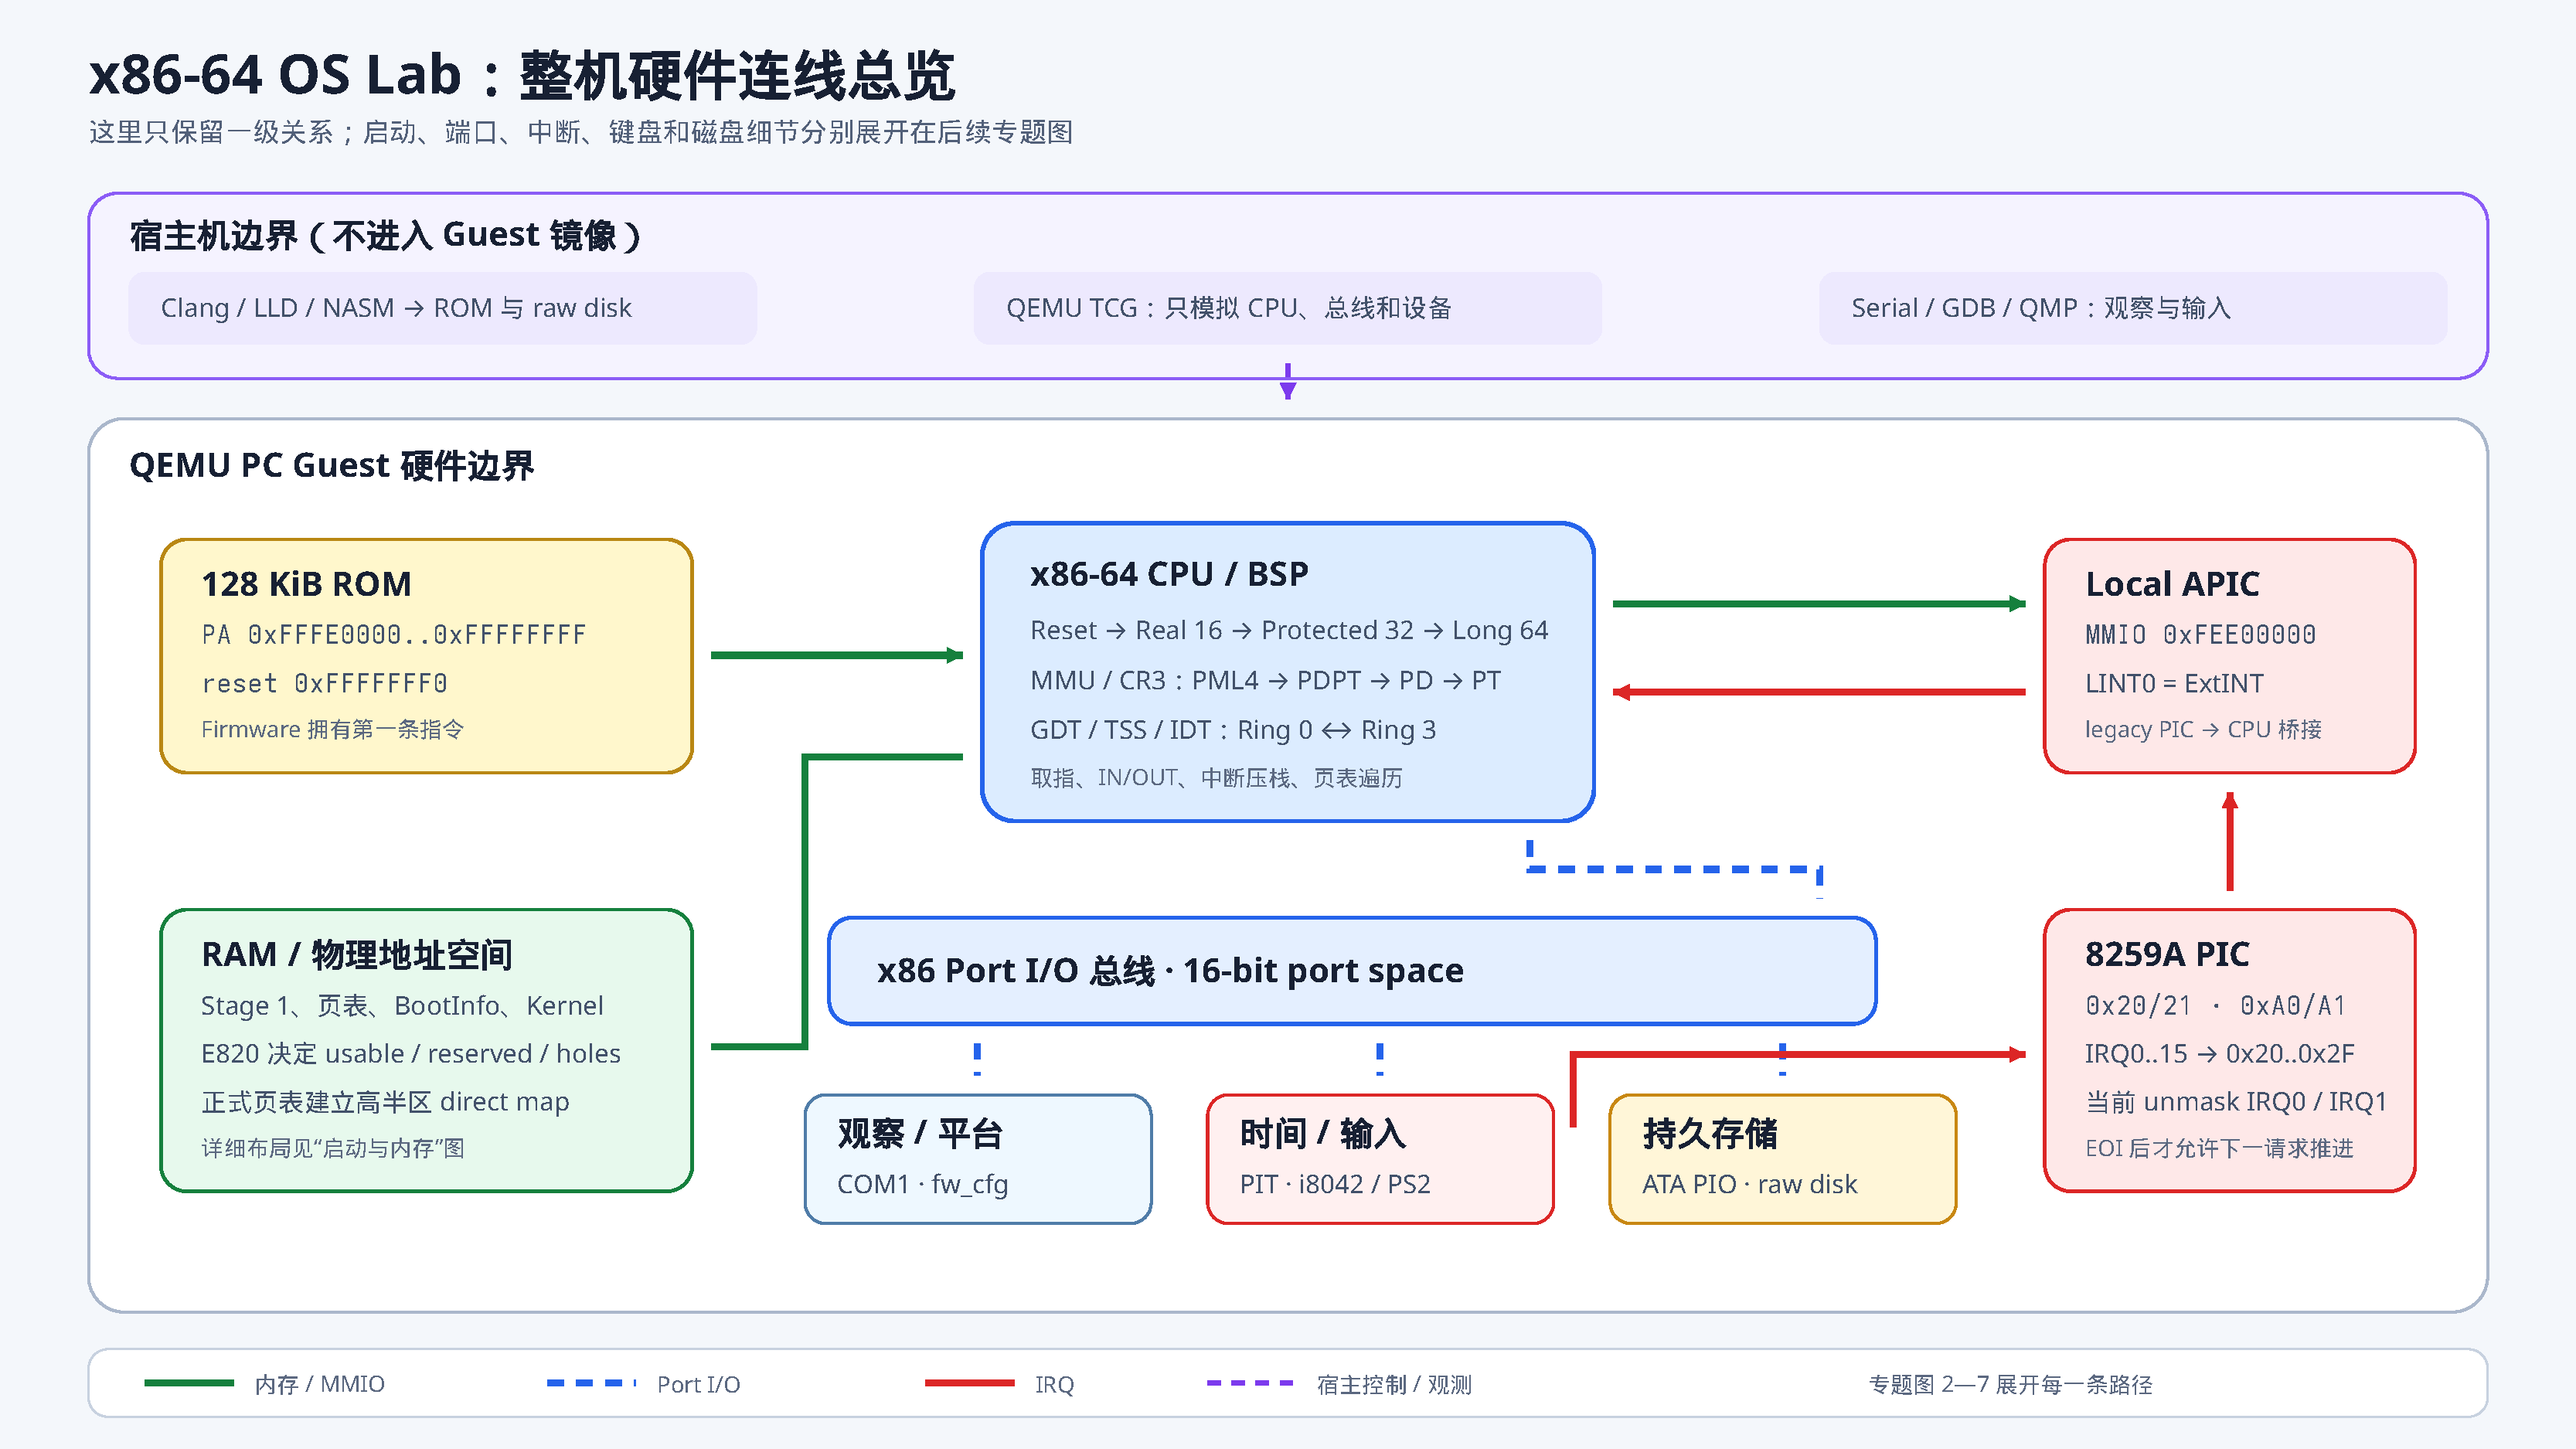
\includegraphics[width=0.96\textheight,height=0.82\textwidth,keepaspectratio]
    {figures/system_wiring/x86_64_os_hardware_wiring.pdf}
  \caption{STUOS 整机硬件连线总览。图中文字、线条和箭头均为矢量对象；
  横置整页用于保留可读字号。绿色、蓝色、红色和紫色分别表达不同事务，
  不能把它们当作一束同类导线。}
  \label{fig:system-wiring-overview}
\end{sidewaysfigure}
\clearpage

\subsection{三、沿整机总览逐块理解硬件}

\subsubsection{3.1 Host 为什么画在 Guest 外面}

\term{Host}{宿主}是运行构建工具和 QEMU 的现有系统；
\term{Guest}{客户机}是 QEMU 模拟出来、供 STUOS 使用的目标机器。Clang、
LLD、NASM 和镜像工具在宿主执行，产出 ROM 与 raw disk；它们不会随产物进入
客户机。Serial、GDB 和 QMP 也是宿主观察/控制接口，但它们观察的是客户机
状态或向设备模型提交事件。

QEMU TCG 位于宿主软件中，却对客户机实现 CPU、地址空间和设备规则。这里有
两个同时正确的描述：

\begin{itemize}[leftmargin=2em]
  \item 从宿主实现看，QEMU 是一个普通进程，设备模型是 C/C++ 代码；
  \item 从 STUOS 看，QEMU 提供的 ROM、RAM、PIC 和 ATA 就是它实际面对的硬件
        契约，目标代码不能直接调用宿主库跳过寄存器协议。
\end{itemize}

\subsubsection{3.2 ROM、RAM 和磁盘为什么画成三个部件}

ROM 保存断电后仍存在的最早固件字节，并被平台映射到复位可取指地址；RAM
保存运行时栈、页表、BootInfo 和已装入代码；磁盘保存按 LBA 编号的持久扇区。
CPU 可以直接从已映射 ROM/RAM 取指，却不能把 ATA 扇区号当作 RIP。完整搬运
路径是：
\[
\text{disk sector}
\rightarrow \text{ATA data register}
\rightarrow \text{CPU register}
\rightarrow \text{RAM}
\rightarrow \text{instruction fetch}.
\]

总览中的绿色线把 ROM、RAM、CPU 和 Local APIC 放在物理地址/MMIO 一侧，
并不意味着三者电气相同。ROM 拒绝普通写入，RAM 可读写，Local APIC 寄存器
具有副作用；平台地址译码只是在同一个地址事务入口上把范围分给不同响应者。

\subsubsection{3.3 CPU 方框为什么同时出现 MMU、描述符表和 Ring}

CPU 不只做算术。MMU 根据 CR3 和页表翻译地址；GDT/TSS/IDT 给特权转换和事件
入口提供处理器可验证的数据结构；RIP/RSP/RFLAGS 与控制寄存器共同决定下一条
指令在哪里、使用哪个栈、是否接受可屏蔽中断。这些结构多数存放在 RAM 中，
CPU 寄存器只保存入口、根地址或当前选择状态。

\subsubsection{3.4 Port I/O 总线是架构空间，不是一根现代排线}

图中央的 Port I/O 粗线把 COM1、PIT、i8042、ATA 和 PIC 汇在一起，表示它们
都由 \code{IN}/\code{OUT} 指令和 16 位端口号访问。真实芯片内部可由不同片上
互连或兼容逻辑实现；QEMU 则由各设备模型响应相应端口。粗线是软件可见接口的
集合，不宣称主板上存在一根标着“Port I/O”的铜排。

\subsubsection{3.5 PIC 与 Local APIC 为什么同时存在}

8259A PIC 接收传统 IRQ0/IRQ1，经过初始化后把它们映射为向量
\code{0x20}/\code{0x21}。本项目使用 virtual-wire 路径把 PIC 的 INTR
经 Local APIC LINT0/ExtINT 交给 BSP。蓝色端口线用于配置 PIC，红色 IRQ
线用于报告事件，绿色 MMIO 线用于配置 Local APIC；三条线共同存在才构成
完整中断路径。

\subsection{四、路线图不是版本纪念册，而是依赖图}

\begin{sidewaysfigure}[p]
  \centering
  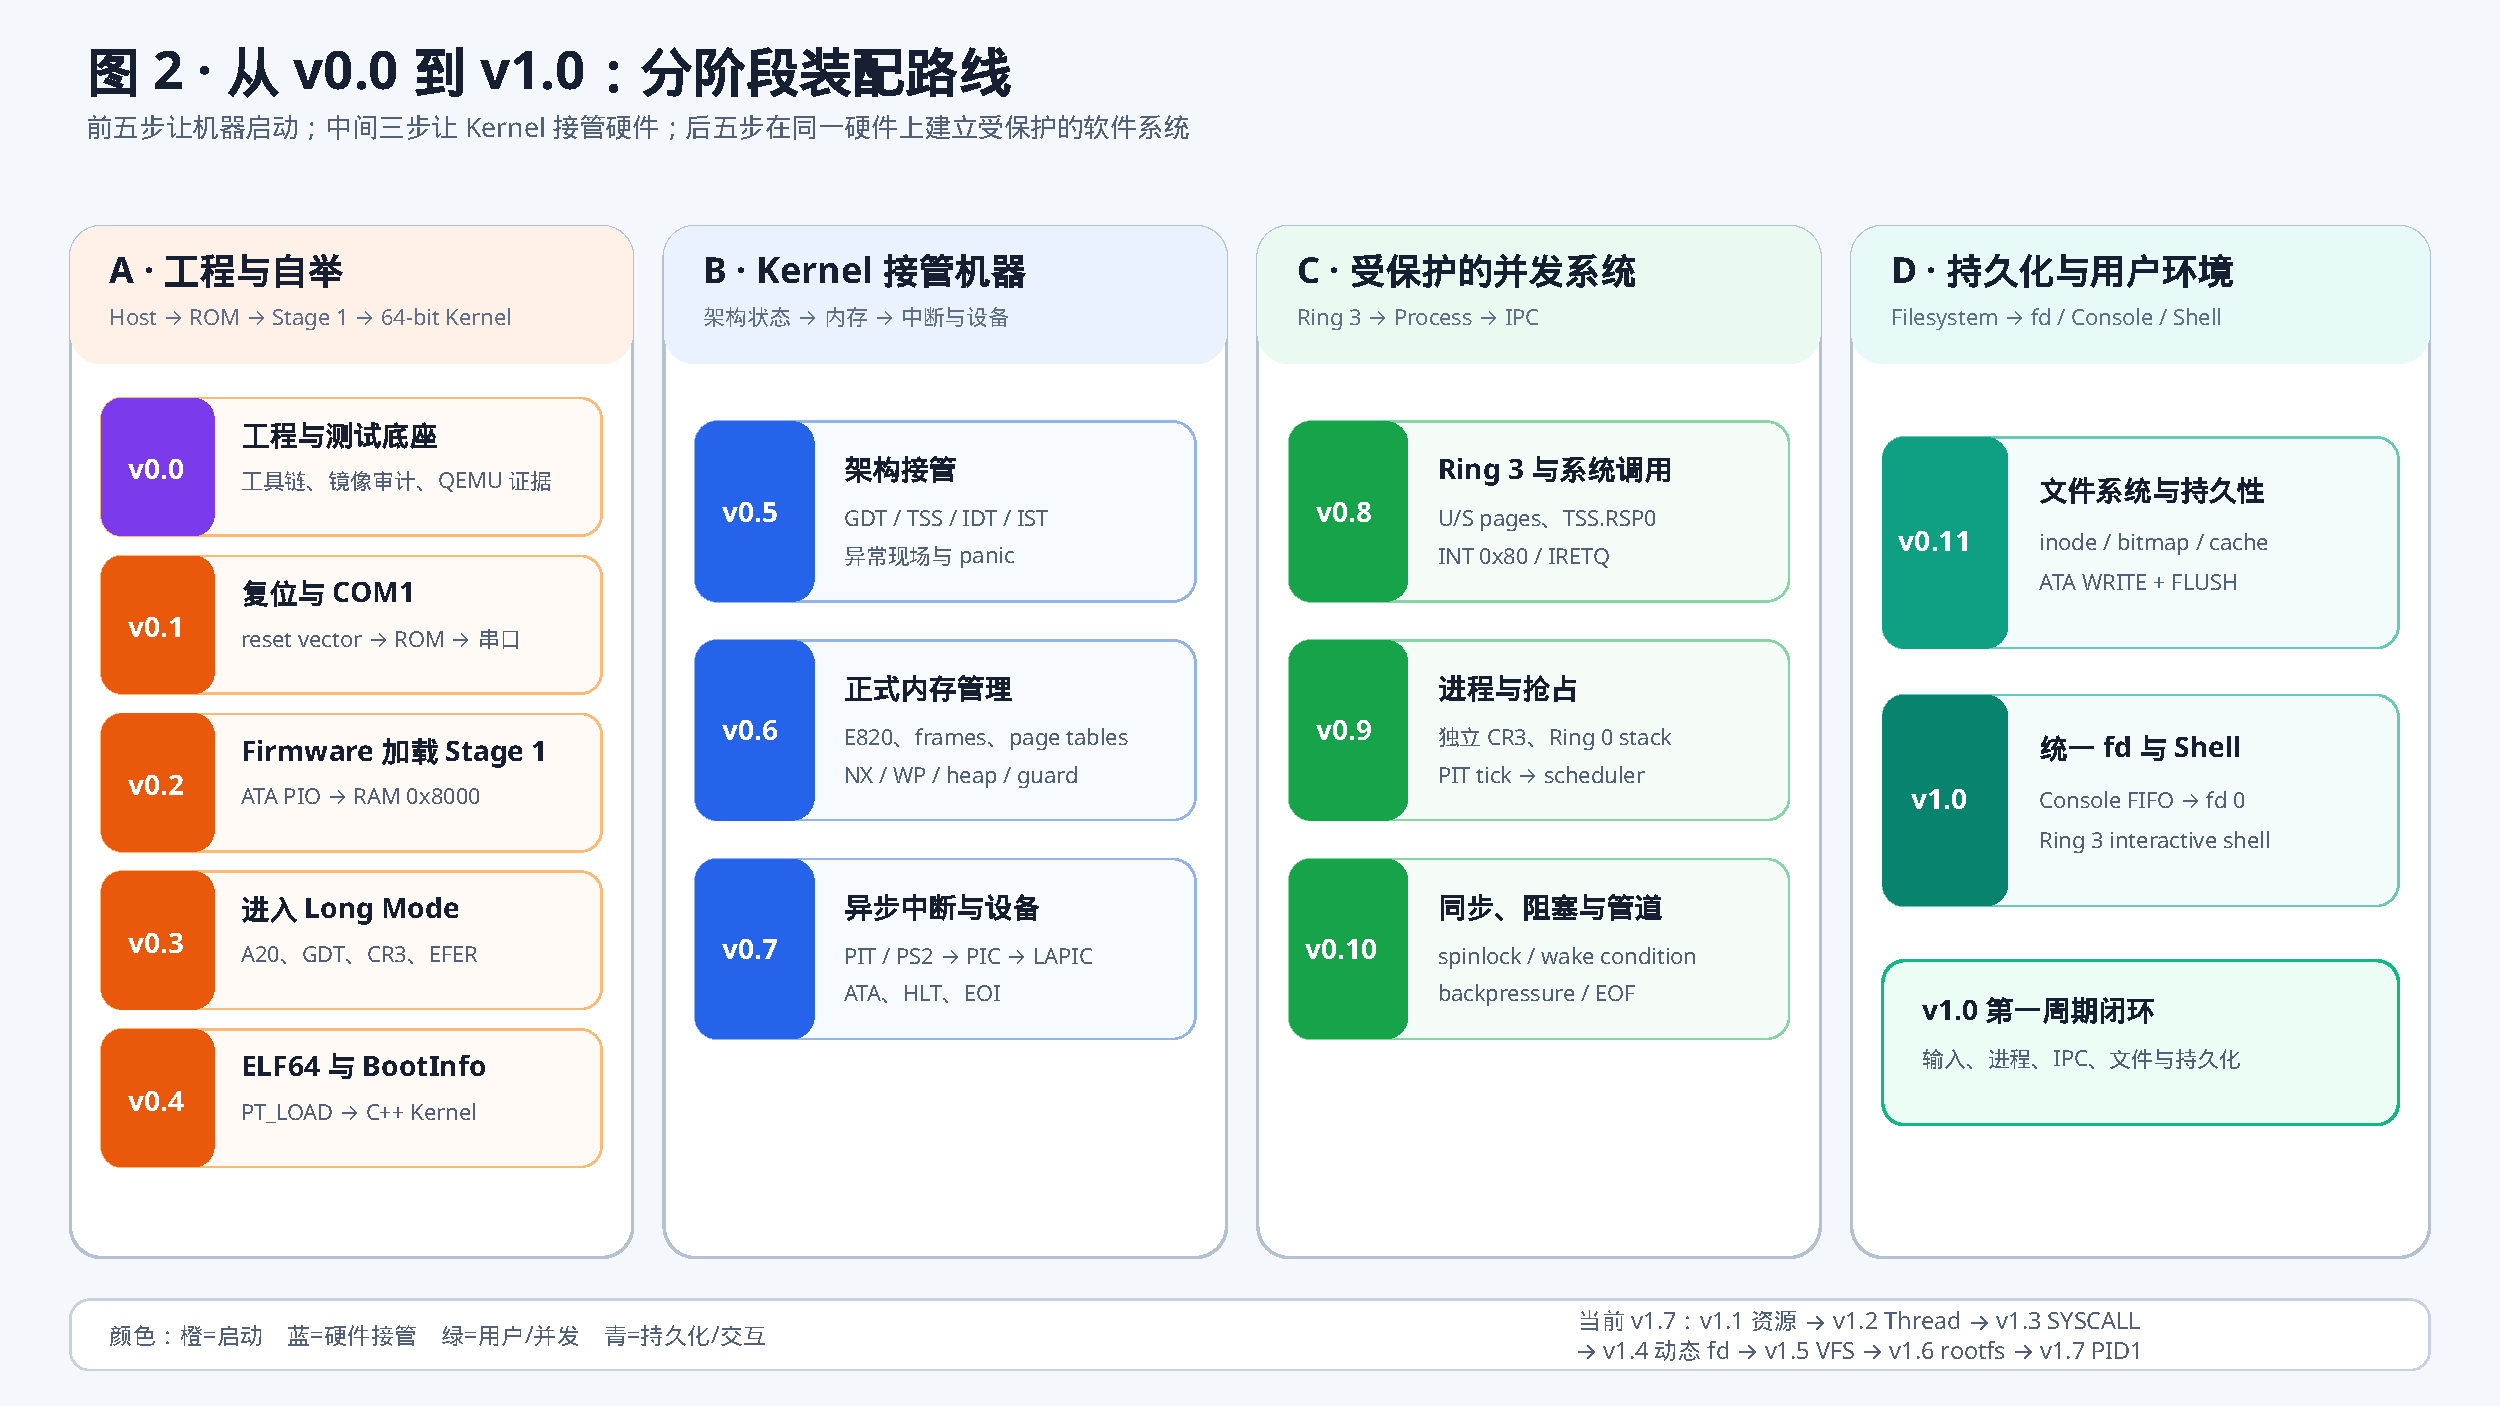
\includegraphics[width=0.96\textheight,height=0.82\textwidth,keepaspectratio]
    {figures/system_wiring/hardware_stage_roadmap.pdf}
  \caption{从 v0.0 到 v1.0 的十三个可验收增量。每张卡片表示新建立的一组
  前置条件；箭头方向是能力依赖，不表示后续版本删除旧机制。图下方同时标明
  当前 v1.1--v1.6 的资源、Thread、SYSCALL、动态文件表、VFS 与 rootfs v2 增量。}
  \label{fig:hardware-stage-roadmap}
\end{sidewaysfigure}
\clearpage

路线图把第一周期分成四组，不是为了按颜色记忆，而是为了防止同时打开太多
不可观测状态：

\begin{longtable}{L{0.14\linewidth}L{0.21\linewidth}L{0.30\linewidth}L{0.25\linewidth}}
\toprule
阶段 & 增量 & 新获得的能力 & 为什么不能提前 \\
\midrule
A 工程与自举 & v0.0--v0.4 & 可复现构建、ROM、串口、Stage 1、长模式、ELF 与 BootInfo & 没有前一层便无法观察或装入后一层 \\
B Kernel 接管 & v0.5--v0.7 & GDT/TSS/IDT、物理内存、页表、异常、中断和设备 & 内核先要能隔离故障，才适合接受异步事件 \\
C 受保护并发 & v0.8--v0.10 & Ring 3、系统调用、进程、抢占、阻塞与 IPC & 用户边界依赖页权限、内核栈和异常入口 \\
D 持久化与交互 & v0.11--v1.0 & 文件系统、统一 fd、控制台与 Shell & 交互命令要依赖调度、驱动和持久对象的完整链 \\
\bottomrule
\end{longtable}

\topic{“后续能力”不会让早期硬件消失}%
v1.0 的 Shell 打印一个字符，仍要依赖 v0.1 建立的 UART；读取文件仍要依赖
v0.2 开始使用的 ATA；进入 Ring 3 仍要依赖 v0.3 的模式转换和 v0.5 的
描述符表。版本号表达的是第一次建立某项能力，不是该能力只在那个版本存在。

\topic{v1.1--v1.6 为什么画在第一周期之后}%
v1.1 收口可回收内核资源，v1.2 把 Process 与 Thread 分离，v1.3 加入原生
SYSCALL/SYSRET 与 CPU-local，v1.4 建立类型化 KernelObject、共享
FileDescription 和动态 FileTable，v1.5 再建立 VFS、挂载与 memfs，v1.6
则让 rootfs v2 承担可扩展持久化与完整命名空间修改。它们在
v1.0 已闭合的启动、用户、文件和
测试链上继续强化生命周期与接口，不改写“先有机器状态，后有软件抽象”的依赖
方向。

\subsection{五、读任意一张硬件学习图的七问法}

后续看到更复杂的图，可以逐节点回答七个问题：

\begin{enumerate}[leftmargin=2.2em]
  \item 这个框是物理器件、架构状态、软件对象，还是宿主工具？
  \item 输入从哪里来，输出到哪里去，方向是否会反转？
  \item 线表示数据搬运、控制流、地址事务、中断请求，还是测试控制？
  \item 这一步由固件、引导器、内核、驱动还是用户程序初始化？
  \item 完成条件由哪个状态位、寄存器、返回值或测试标记证明？
  \item 失败时数据还归谁，是否需要回滚、清中断、释放内存或保持磁盘不变？
  \item 把 QEMU 换成实体平台后，哪个接口保持，哪个地址、设备或固件假设必须
        重新发现？
\end{enumerate}

如果七问中有一项只能回答“反正箭头连着”，说明图还没有读成工程契约。后续
六张整机专题图会分别把启动/内存、Port I/O、中断、键盘和持久化路径放大，
第二章实体案例再把电源、差分对和引脚真正落到 PCB 网络。

